\documentclass[11pt,twoside]{report}
\usepackage[a4paper,width=160mm,top=20mm,bottom=20mm,bindingoffset=6mm]{geometry}

\usepackage{amsthm}
\usepackage{amsfonts}
\usepackage{amsmath,amssymb}
\usepackage{graphicx}
\usepackage{wrapfig}
\usepackage[T1]{fontenc} 
\usepackage[utf8]{inputenc}
\usepackage{graphicx}
\usepackage{wrapfig}
\usepackage{mathtools} 
\usepackage{lipsum}
\usepackage{color}
\usepackage[english]{babel}
\usepackage{appendix}
\usepackage{float}
\usepackage{enumitem}
\usepackage{setspace}
\usepackage{subcaption}
\usepackage{amssymb}
\usepackage{fancyhdr}
\usepackage{titlesec}
\usepackage{mathrsfs}
\usepackage[ruled,vlined]{algorithm2e}

\titleformat{\chapter}[display]
{\normalfont\huge\bfseries}{\chaptertitlename~\thechapter}{20pt}{\Huge}
\titlespacing*{\chapter}{0pt}{30pt}{15pt}
\titlespacing*{name=\chapter,numberless}{0pt}{-30pt}{10pt}

\newenvironment{system}
{\left\lbrace\begin{array}{*{4}{c@{}>{{}}c<{{}}@{}}c}}
	{\end{array}\right.}
\setlength{\parindent}{0pt}

\makeatletter
\@addtoreset{section}{part}
\makeatother
\renewcommand{\partname}{}
\linespread{0.75}
\newcommand\independent{\protect\mathpalette{\protect\independenT}{\perp}}
\def\independenT#1#2{\mathrel{\rlap{$#1#2$}\mkern2mu{#1#2}}}
\let\oldemptyset\emptyset
\let\emptyset\varnothing
\singlespacing
\newtheorem{definition}{Definition}
\newtheorem{lemma}{Lemma}
\newtheorem{prop}{Proposition}
\newtheorem{model}{Model}

\begin{document}
	
\pagenumbering{gobble}
\vspace*{-1.5cm}{
	\begin{center}
		\large
		POLITECNICO DI MILANO\\
		\normalsize
		Master Degree in Mathematical Engineering\\
		Industrial and Information Engineering\\
		Department of Mathematics\\
		\begin{figure}[htbp]
			\begin{center}
				
\includegraphics[width=3.5cm]{./pictures/logo.jpg}
			\end{center}
		\end{figure}
		\vspace*{0.3cm} \LARGE
		
		
		
		\textbf{A Bayesian model for data flow: BikeMi}\\
		
		
		\vspace*{.75truecm}\large
		\vspace*{.5truecm} \large
		052499 - Bayesian Statistics Project Short Report
	\end{center}
	\vspace*{3.0cm} \large
	\begin{flushleft}
		
		
		Professor: Alessandra Guglielmi \\
		Professor: Riccardo Corradin \\
		Project Tutor: Mario Beraha
		
	\end{flushleft}
	\vspace*{3.0cm}
	\begin{flushright}
		
		
		Group members:\\
		Andrea De Gobbis \\
		Lorenzo Ghilotti \\
		Giorgio Meretti
		
		
	\end{flushright}
	\vspace*{2.0cm}
	\begin{center}
		
		
		
		Academic Year 2019-2020
	\end{center} \clearpage
}
\shipout\null

\pagenumbering{arabic} 
\pagestyle{fancy}
\fancyhf{}
\fancyhead{}
\fancyhead[RO,LE]{BikeMi -- add}
\fancyfoot{}
\fancyfoot[C,C]{\thepage}
\renewcommand{\headrulewidth}{0.4pt}

\tableofcontents{}

\chapter*{Introduction}
This project is the natural continuation of the work due to G. Bissoli, C. Principi, G. M. Rinaldi (BG19 in the bibliography), last year. But, whilst their goal was that of predicting the amount of traffic in a network independently of the particular day in which data have been registered, our main purpose will be developing a time series approach to the problem. We will obviously take advantage of some tools, like DBSCAN clusterization, already employed by our colleagues, but every time with a critical aproach, aiming to improve and possibly generalize the baseline already provided to us.\\
\\
In our project we will mainly focus on two targets: developing a global model able to predict the overall amount of traffic in the BikeMi network of Milan, being suitable for daily forecasts, and attempting to produce a network model to mimic the same ideas on the specific graph-based context. In light of these purposes, we will use fully Bayesian tools like loglinear models, Bayesian Structural Time Series (BSTS), spatial approaches and also some heuristics, like the penalized DBSCAN, to fasten computions. We don't have the ambition to produce outstanding results, given the relatively small amount of data at our disposal, but we hope - at least - to provide an introductory insight to the problem, possibly suggesting some methodological patterns and clever ideas to evolve models in this framework.

\chapter{Data preprocessing}
As already pointed out during the introduction, the data preprocessing performed in the original paper - that from now on will be addressed as Model Zero (M0) - was conceived like an elementary preliminary tool capable of creating a shrunk, tractable number of macro-nodes, vital precondition for the feasibility of an on-network Bayesian approach. However, the clusterig operation, carried out with the popular density-based frequentist algorithm DBSCAN, highlighted some critical issues. As an introductory challenge for our project, we tried to improve the design of this early phase, developing a more contextualized - but still frequentist - version of the DBSCAN, in order to better capture the core-periphery structure of big round cities.

\section{Criticalities of a purely Euclidean DBSCAN}
Unquestionably, the primary goal of a location-based clustering is that of grouping  together nodes according to some spatial criterion. The pure DBSCAN identifies the proximity of two nodes using their Euclidean distance and merges multiple locations. In principle, such a method may appear perfectly valid, but unfortunately it seems to overlook a crucial property of a spatial networks: the topology. When dealing with big cities, like Milan, there are some centers of interest which can't be totally neclected, since they tend to aggregate around them a massive traffic and, as a consequence, a bigger number of stations. However, indiscriminate gruping increases considerably the risk of losing both interpretability of the streams and predictive potential. In light of this, we looked at the issue of employing something different from a common notion of distance, to better classify the closeness of two points in a net. To support our thesis concerning the partial inadequacy of M0, we have collected some quantities ponting out the problem, for instance, loop percentage and cluster dimensions, see full report for futher detail.

\section{Penalized DBSCAN}
In this section we are going to present an upgraded version of the classic DBSCAN structure that we decided to employ in order to clusterize the nodes, both covering the main modifications.

\subsection{The algorithm}
The basic idea employed in our work was that of feeding the DBSCAN algorithm with a similarity matrix produced, not by the standard Euclidean distance (denoted by $ ||x-y|| $, $ \forall x, y \in \mathbb{R}^2 $), but with a penalized vesion of it: $ smd(x,y) = \frac{p(y)+p(x)}{2}||x-y|| $, through a suitable non-negative function $ p(*) $. The flexibility of the model is given by the freeedom of choice in the penalization, that we constructed in order to be adapted to a circular-shaped metropolis, like the city of Milan. The goal was that of forcing the DBSCAN algorithm to be more thrifty in the citycenter, to avoid overaggregation around the main monuments and business locations, whilst stimulating, on the other hand, a stronger clustering in periphery. Thus, a straightforward idea was that of a penalization function actually depending from the Euclidean distance between a certain node and the city center (identified by the exact geographical coordinates of the cathedral, $ x_0 $): i.e. $\exists g:[0,+\infty)\rightarrow[0,+\infty)$, non-increasing s.t. $p(x) = g(||x-x_0||),\ \forall x \in \mathbb{R}^2$. We opted for a parametric family of functions for $ g $, able to cover a wide-enough variety of shapes:
\begin{equation}
 g(u) = \max\{\beta, e^{(\frac{u}{\alpha})^2\log{(1-\gamma)}}+\gamma\}\ \ \forall u \in [0,+\infty)
\end{equation}
where $ \alpha>0,\ \beta\in[0,1],\ \gamma \in (0,1) $. In order to make some automatic parameter selection without losing both the constraints and the magnitude $ \mathcal{O}(1) $ defined before, we decided first to normalize $ smd(x_i,x_j),\ \forall i,j \in {id}^2$ with the median of the distances between all the nodes and $ x_0 $, $ m=qt(||X -x_0||,0.5) $, defining $ smd'(x_i,x_j)=\frac{smd(x_i,x_j)}{m} $. Then, given this notion of similarity, it was possible to fix the penalization parameters on uniform grids of step $ \sim \frac{1}{20} $ of the correponding scale factor. Since we were trying to establish the values for which the spatial aggregation best captured the net topology, to automatize the procedure, we decided to restrict the feasible models to a smaller subset of parametric combinations satisfying some minimal requirements $ \mathcal{C} $: weighted loop percentage $ P<15\% $, number of clusters $nc >40 $, percentage of singletons $ I<33\% $. Finally, we defined an empirical goodness-of-fit function $ GOF(m)=P(m)+3I(m) $ for each model $ m $, adapted to the expected optimal sizes of clusters, whose minimization selected the best parametric set as $ \hat{m}=\arg\min GOF(m) $.

\subsection{Results}
The model selected through the penalized DBSCAN has $ \alpha=0.8, \gamma=0.5 $. Since small values of $ \beta $ appear reasonable, we decided to force $ \beta=0 $ 

\begin{algorithm}[H]
	\SetAlgoLined
	Fix a center $ x_0 $;\\
	Fix $ \varepsilon=1.15 $;\\
	Compute $ m=t(||X -x_0||,0.5) $;\\
	\For{$ \alpha \in $ 0.1\ :\ 0.05\ :\ 0.9}
	{
		\For{$ \beta \in $ 0\ :\ 0.05\ :\ 1}
		{
			\For{$ \gamma \in $ 0.1\ :\ 0.05\ :\ 0.9}
			{
				 Compute penalization $ p(x) = \max\{\beta, e^{(\frac{||x-x0||}{\alpha})^2\log{(1-\gamma)}}+\gamma\} $ for each node $ x $;\\
				 Define matrix $ smd'(x,y) = \frac{p(y)+p(x)}{2}\frac{||x-y||}{m} $ for each node couple $ (x,y) $;\\
				 Compute DBSCAN($ sdm' $), 2, $\varepsilon$);\\
				\eIf{$ C $ is $ \mathtt{true} $}{
					Save iteration;\\
					Compute $ GOF(\alpha,\beta,\gamma) $;
				}{
					Discard iteration;
				}
			}
		}
	}
	Select $ (\hat{\alpha},\hat{\beta},\hat{\gamma})=\arg\min GOF(\alpha,\beta,\gamma) $;\\
	\KwResult{Clusterization of the nodes in a graph}
	\caption{Penalized DBSCAN}
\end{algorithm}

In order to improve the performance given by M1, a sensible subdivision of cluster 1013 seemed unavoidable. Indeed, there were strong topological reasons to consider that merging improper and, as a final consideration, just notice that the contribution to the total weighted loop percentage $ P_1=4.72\% $ given only by 1013 was $ 1.54\% $. Almost $ 1/3 $ of the improper aggregation of the net was located in this single macro-cluster! Since $ P_{1013}^1=18.78\% $, a separation in 2 or 3 subsets seemed - a priori - to be the right choice. This intuition found confirmation in the results. Given $ \hat{\alpha}=0.8,\ \hat{\beta}=0,\ \hat{\gamma}=0.5 $ as in the previous subsection, we decided to tune locally the penalized DBSCAN, playing a bit with the value of $ \varepsilon $, restricted to the mere region 1013. Calling the model disaggregating the macro-group as M2, we found a clusterization structure with only the $ 4\% $ of weighted loops and strongly topologically adherent with the original network. 

\section{Iterated Penalized DBSCAN}
In order to force the aggregation of some more isolated point, reduce the computational complexity of the Bayesian study and finally attain a more uniform spatial layout closer to Milan viability, we proposed one last modification to the already implemented corrected penalized DBSCAN M2. The main variation in model M3 - as will be denoted form now on - consisted in the addition of a second layer of penalized DBSCAN to the already proposed spatial grid. Dividing the clusterization in two phases partially resolves some problems of aggregation. Indeed, it allows to first compute the most interconnected sets and then substitute them with their ideal Euclidiean baricenters - a reasonable approximation of their penalized equivalents, for which lacks a rigorous definition. In particular, letting first layer clusters collapse on their baricenters somehow makes them "less attractive" for the second iteration; in the sense that, in principle, a reasonably large penalized neigbourhood without any station in proximity should be created around any of them, at least in case of proper clustering. Conversely, in case of missed points, the algorithm will tend to incorporate more easily the lost singletons in the area, thus stimulating the clusterization of the remaining units. See figure \ref{fig:comparison} for our final result.
\begin{figure}[H]
		\centering
		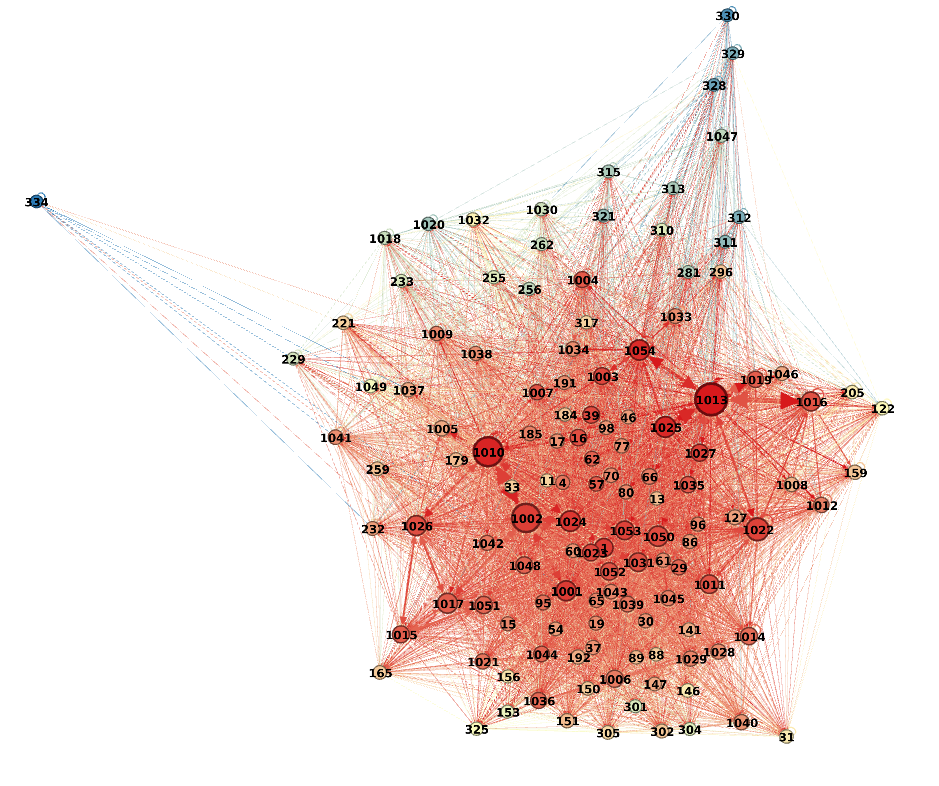
\includegraphics[width=100 mm]{pictures/M2_graph.png}
		\caption{Model M2}
	\label{fig:comparison}
\end{figure}
 One might ask itself if adding more iterations would not improve even further the aggregation. It depends, but in general no, since repeating too much the procedure may amplify the difference between penalised and Euclidean baricenters, originating improper overaggregation more frequently. In this particular case, even a third layer of clustering is not very effective, if not detrimental. As a conclusion, it's worth starting from the weighted loop percentage of the net, which has always been the simplest way to measure the goodness-of-fit of a clustering w.r.t. the true hidden topology. By hypothesis $ P_3\geq P_2 $. The issue lied in how great the difference was. Luckily a tolerable quantity: just $ 4.35\% $: starting from a benchmark of $ 3.99\% $; note this quantity to be still smaller than M1's average weighted loop percentage. Moreover, this estimate can also be considered quite robust, since the only outliers - i.e. stations over the $ 10\% $ in loop percentage - are the already well known extreme nodes 330, 334 and 1047, plus Central railway station cluster 1013, with a value of $ 10.53\% $, slightly out of the bounds. Moreover, we selected the threshold for having an hub at the usual $ 10000-12000 $ links which amounts to $ 2000 $ departures/week. The sole clusters able to surpass this limit were 1002 (Cadorna station), 1010 (Sempione), 1013 (Central station), 1022 (Viale Indipendenza-Via dei Mille), 2006 (Cordusio). However their loop percentages is still under control: $ 1.3\%,\ 9.48\%,\ 10.53\%,\ 7.16\%,\ 2.9\% $.


\chapter{Frequentist preprocessing}
The main goal of this report is suggesting strategies to predict the traffic of the BikeMi network in Milan. In order to achieve this goal, we will follow two distinct, but complementary, paths: a global analysis whose main aim is finding a way to forecast the overall amount of trips that will be carried out during a well specified day, and a network analysis where we want to determine the global number of trips started or ended in the macro-nodes generated through the corrected DBSCAN preprocessing, that we have mentioned before. In both cases our main purpose is using models which are feasible enough from the computational viewpoint to allow, without a big loss in terms of precision, the realization of forecasts in a maximum time span of one day.

\section{Data representation}
Since dealing with a problem of traffic concerning light vehicles, atmospherical conditions have been examined in order to find some interplay with the variation in the number of bikes on the net. In the following graph, we show a qualitative comparison in the effect of rain, wind, humidity and temperature with the overall amount of bikes in a day. Unfortunatey, the data available for $ 2016 $ share a daily horizon, thus we can't have a precise division in time slots for a more refined type of analyis. Nonetheless, we will try to disagregate the study also in time zones, struggling to capture the discrepancies in volume through other strategies typical of structural time series.

\begin{figure}[H]
		\centering
		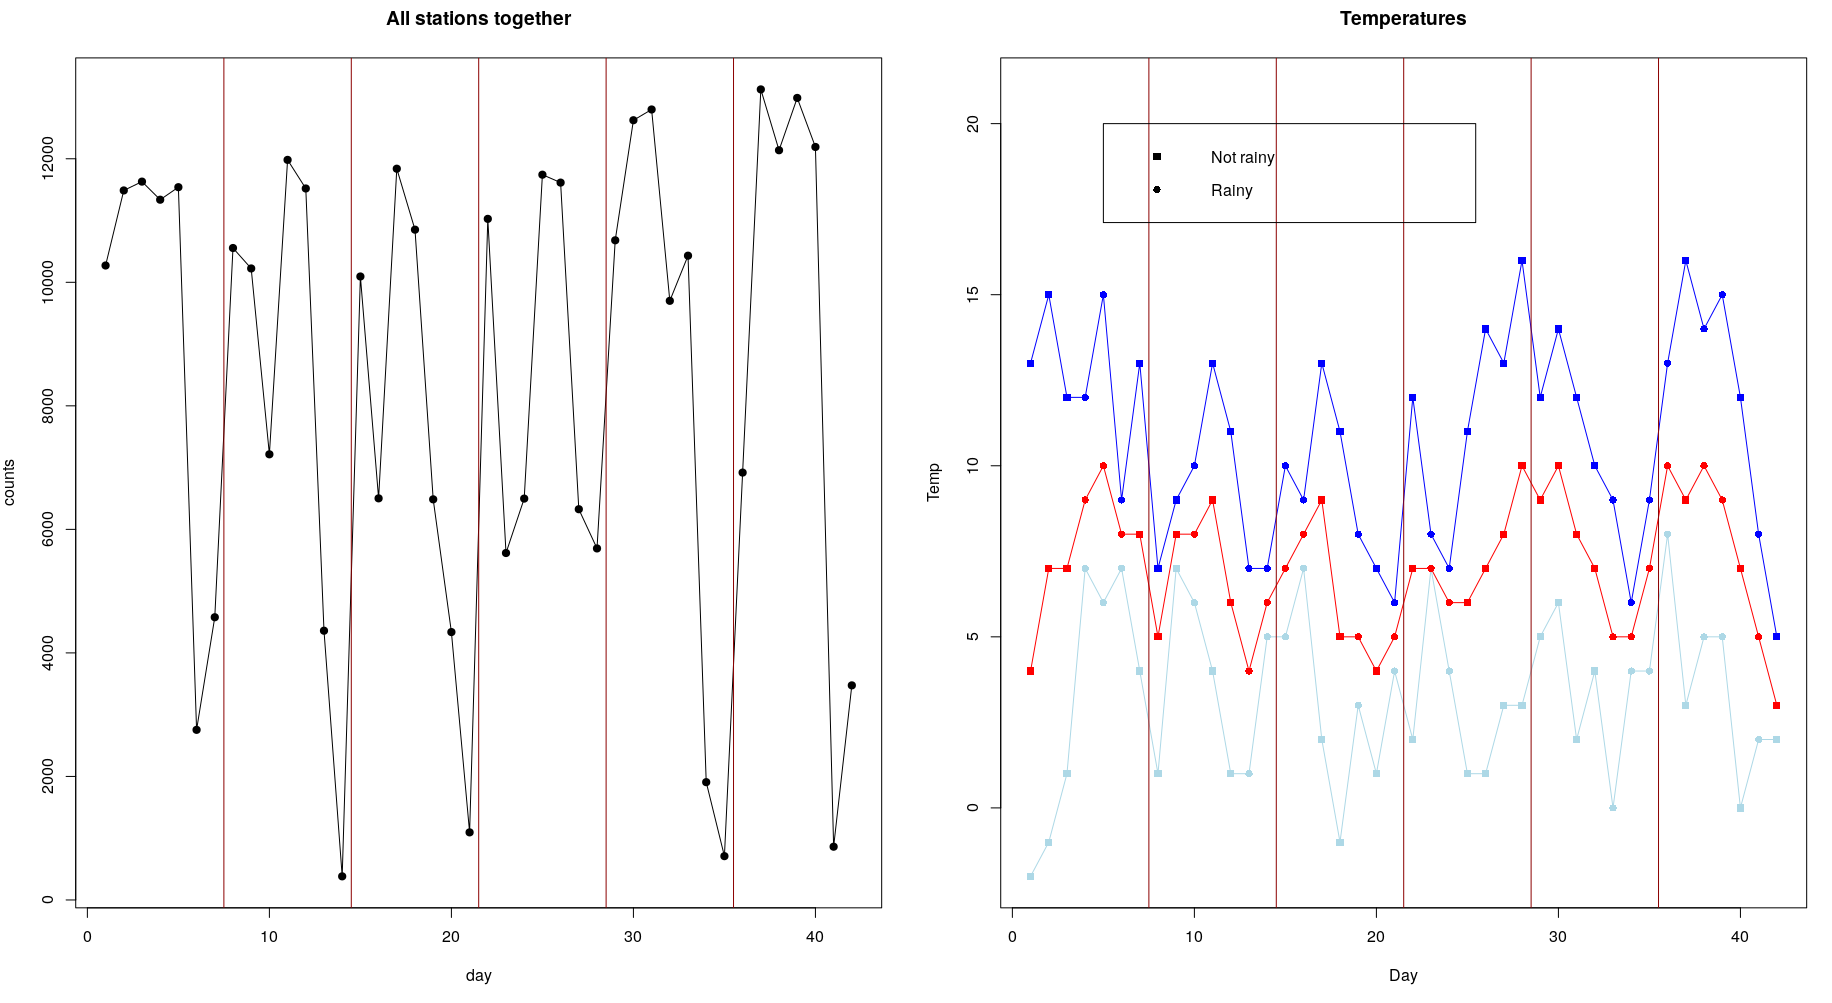
\includegraphics[width=110 mm]{pictures/temperatures.png}
		\caption{Temperatures}
		\label{fig:temperature}
\end{figure}

As for the moment just observe that there does not appear to be a strong relationship between traffic and humidity or wind, while on the opposite temperature seems sometimes proportional to the effective output. A bit different is the nature of rain. Even though the time series seems to have a natural periodicity, the action of rain sometimes disrupts this behaviour, since the number of bikes drops abruptly in correspondence of strong phenmena.  This easily meets intuition. Motivated by these results, we will try to use the two factors as predictive tools in the future.

\section{Stationarization}
In order to check the possibility to consider our model as a structural time series, we decided to employ a frequentist moving average + periodicity filtering, a second goal will be that of verifying the stationarity of the found residuals. The idea behind the stationarization is substantially the following: each datum can be seen as the sum of a trend represented by a moving average, a periodic component repeating itself identical during the various weeks and a residual effect: in principle a stationary process (for instance a white noise or an ARMAX paradigm): $ y_t = m_t + s_t +r_t $ where $ m $ is the m.a., $ s $ period and $ r $ residual. To produce these estimates we employed the following pre-codified techniques, described for instance in BD02, see bibliography.\\

\begin{algorithm}[H]
	\SetAlgoLined
	Set the time horizon T and period S;\\
	Set $ q=(S-1)/2 $;\\
	\For{$ i \in $ 1\ :\ T}
	{
		Compute $ m_i $ = $\sum_{j=\max\{-q,0\}}^{\min\{q,T\}} y_{i+j}/S$;
	}
	\For{$ k \in $ 1\ :\ S}
	{
		Compute the average $ w_k $ of the deviations $ \{(y_{k+jS} - m_{k+jS} ),\ q < k+jS \leq T-q\} $;
	}
	\For{$ t \in $ 1\ :\ T}
	{
		Compute  $ s_t = s_{k(t)} = w_k-S^{-1}\sum_{i=1}^{S}w_i $;\\
		Compute  $ r_t=y_t-m_t-s_t $;
	}

	\KwResult{Decomposition $ y_t=m_t+s_t+r_t $}
	\caption{Frequentist stationarization}
	
\end{algorithm}

\begin{figure}[H]
	\begin{subfigure}[H]{0.5\linewidth}
		\centering
		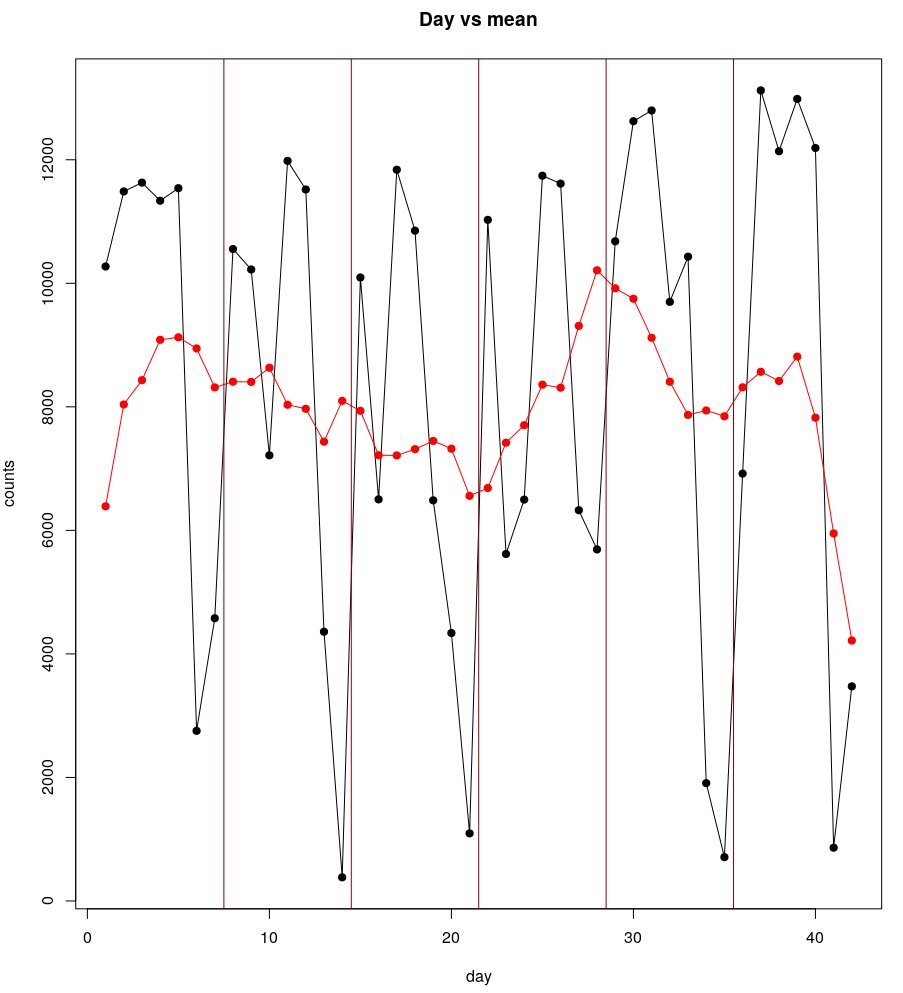
\includegraphics[width=65 mm]{pictures/moving_average.png}
		\caption{Moving average}
		\label{fig:ma}
	\end{subfigure}
	\hfill
	\begin{subfigure}[H]{0.5\linewidth}
		\centering
		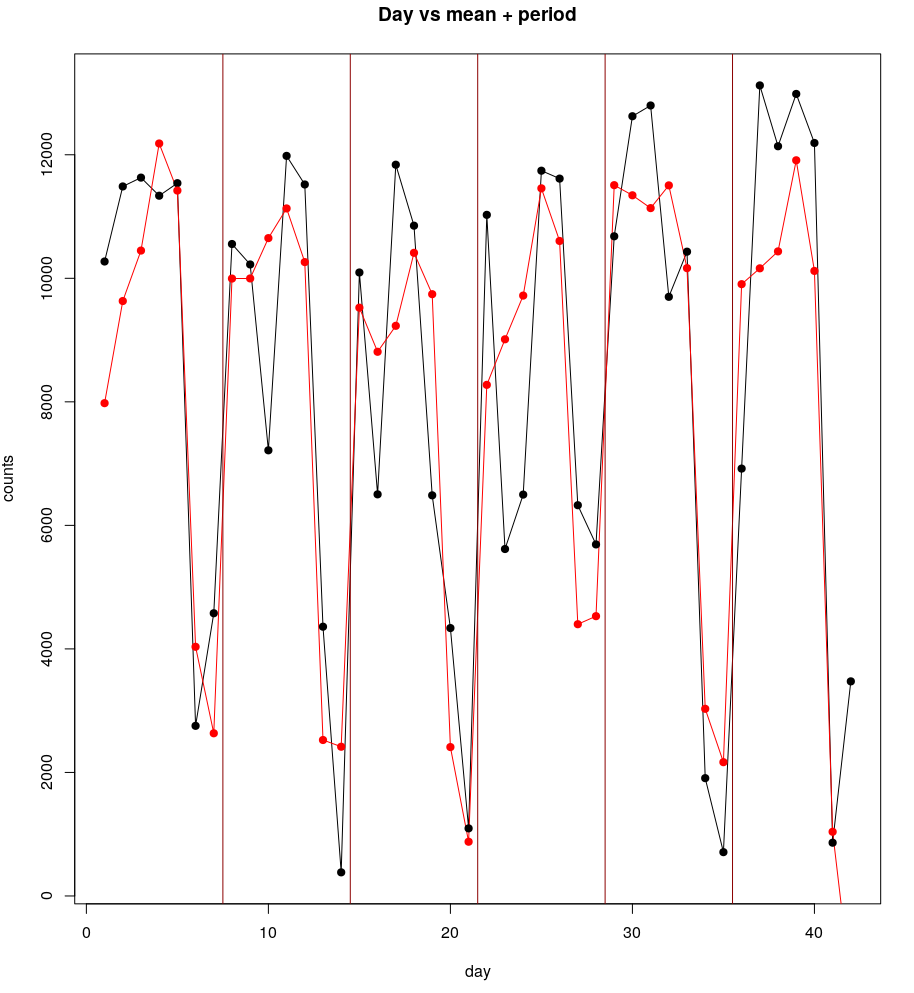
\includegraphics[width=65 mm]{pictures/period.png}
		\caption{Moving average + periodicity}
		\label{fig:period}
	\end{subfigure}
\end{figure}

Note that, apart from the irregularities deriving from the boundaries of the time span where the moving average works not properly well (i.e. the first and last weeks), all the other days show a quite regular trend and the $ m_t+s_t $ term captures already rather well the value of $ y_t $. Just observe also that most of the discrepancies emerge facing rainy days in which there are sudden variations (usually strong falls) with respect to standard behaviour of the historical series. Indeed looking also at the residuals we can see a good oscillating trend mostly negative in rainy days and positive in sunny ones. Moreover, the autocorrelation plot testifies that the residual chain has a white noise $ WN $ behavior. According to most reliable frequentist stationarity tests (Augmented Dickey-Fuller, Phillips-Perron, KPSS) the p-value of having a non stationary chain is less than $ 0.10 $, hence we can quite confidently reject the null hypothesis and postulate the stationarity.

\chapter{Global model}
This chapter will be entirely devoted to the description and comparison among several possible Bayesian models, capable of sinthesizing the total taffic taking place in Milan during a six week long time span occured between January $ 25^{th} $ and March $ 6^{th} $, 2016. The total amount of data available to us consisted of 350,093 trips among stations of the BikeMi network. However, at least for this first part, we will only rely on the day-by-day cumulative traffic, neglecting the graph-specific topology. For further details about the dataset and atemporal analysis please refer to BG19 in the bibliography. Let us just point out the lineup of this chapter before entering into the heart of the modelistic phase: first we will discuss a loglinear strategy to deal with counting data, trying to highlight its usefulness in  covariate selection, but also the limits faced against heterogeneous and highly variable phenomena. Afterwards, we will devote some time discussing multiple Bayesian Structural Time Series approaches, eventually comparing the results with the ones produced by the aforementioned methods.

\section{Loglinear regression}
\subsection{Poisson likelihood}
The most straightforward model for counting data we considered is a loglinear generalized linear model, with Poisson likelihood :
\begin{model} Loglinear GLM with Poisson likelihood\\
	\begin{equation*}
	\begin{aligned}
	&\textsc{Model}\\
	&Y_t  |  \lambda_t \overset{\independent}{\sim} Pois(\lambda_t)\\
	&\log{\lambda_t} = \boldsymbol{\beta}^T\mathbf{z}_t\\
	\end{aligned}
	\qquad \qquad
	\begin{aligned}[c]
	&\textsc{Priors}\\
	&\boldsymbol{\beta} \sim \mathcal{N}_p(\mathbf{0}, \tau \mathbf{I})
	\end{aligned}
	\end{equation*}
\end{model}
Note that from now on normal distributios will be written using precisions. In this first version, moreover, $ \tau=0.001 $ and we take the following covariates:
\begin{itemize}
	\item $Y_{yest}$: volume of traffic during the previous day,
	\item $Y_{an}$: volume of traffic during the same day of the previous week,
	\item $W$: a binary variable representing weekdays or weekends, 
	\item $R_t$: a discrete variable representing the intensity of the rain (from 0 to 9),
	\item $R_{yest}$: analogous to $R_t$ referring to the previous day,
	\item $T$: the mean temperature of the day.
\end{itemize}  

We actually introduced two regression parameters for explaining the effect of $Y_{yest}$: we believe its effect on the next day can depend on the fact that we are on the weekends-weekdays boundary.   
The model is built on 35 observations, as the first week is used for defining the covariates. Results are not good at all, in terms of prediction of the already observed 35 days.\\
\\
Indeed, looking at the 90$\%$ credibility intervals for the $Y_t$ samples for the 35 days, we highlight that these intervals are shorter than what we need: the phenomenon is much more uncertain than what our model is able to describe.
Only 2 observations out of 35 fall inside the credibility intervals.
Having a look also at the distributions of regression parameters, we note that some covariates are irrelevant.
\begin{figure}[H]
	\centering
	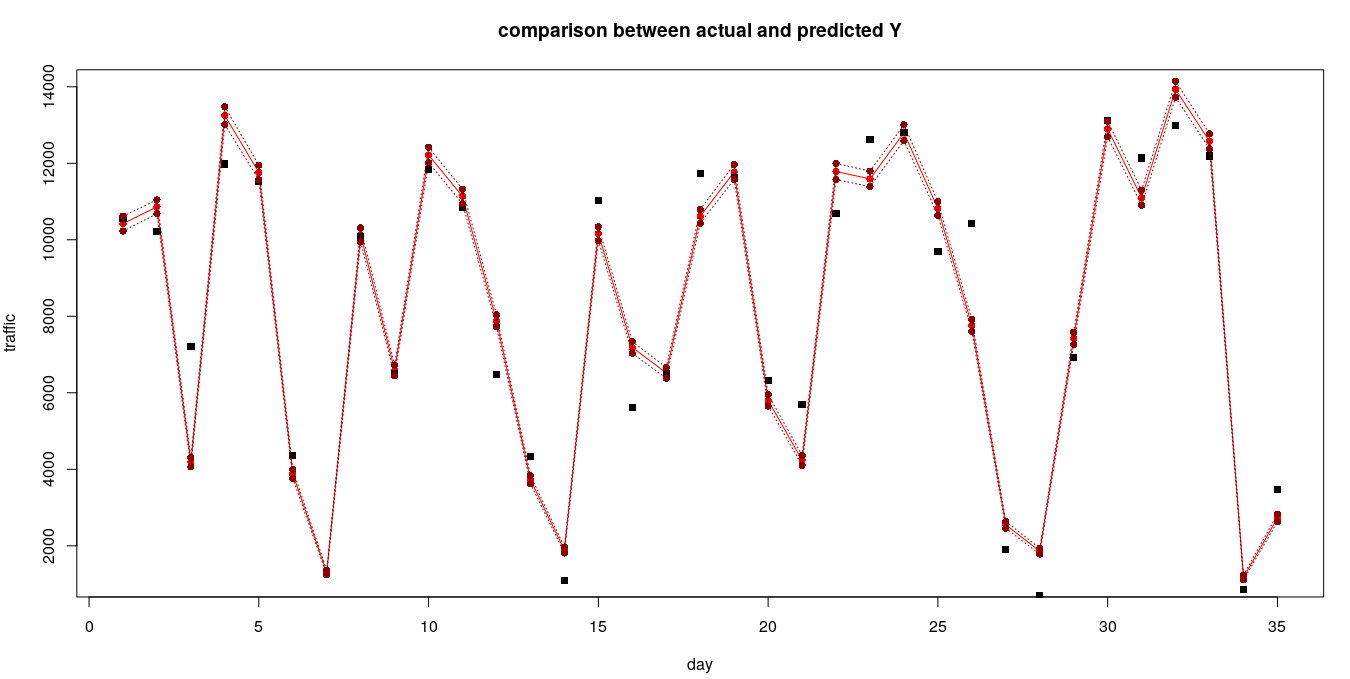
\includegraphics[width=160 mm]{pictures/poiss_y.png}
	\caption{90$\%$ Credibility intervals for $Y_t$ samples}
	\label{fig:poiss}
\end{figure}
Therefore, we tried a Spike\&Slab approach which suggests to remove $Y_{an}$, so we also have a similar model without that covariate. The results, as expected, are similar: the model still suffers the under-estimation of the phenomenon variability. For the previous considerations, we left the Poisson likelihood behind, without further investigating the role of covariates. However, from this initial model we extracted some useful information about the importance of specific variables in explaining the phenomenon: $W$, $R_T$ and $T$ appear influential covariates, and this is coherent with their model-related interpretation.
\subsection{Negative Binomial likelihood}
We needed to overcome the limits of the Poisson likelihood: those problems are related to the presence of a single parameter which determines both mean and variance, and to the fact that our phenomenon is intrinsically more uncertain than the Poisson model is able to describe. Following these observations, we proposed a loglinear generalized linear model with Negative Binomial likelihood. This distribution is described by two parameters, allowing for more flexibility; moreover it comes with an higher variance than its mean, and this could be what we needed.
We refer to the following formulation for the negative binomial density function:
\begin{equation}
f(k;r,p) = \frac{\Gamma(k+r)}{k!\ \Gamma(r)} p^k (1-p)^r \ \ \forall k\in\mathbb{N}
\end{equation}
According to this convention, if $X \sim NegBin(r,p)$, we have $\mathbb{E}[X] = \mu = \frac{r(1-p)}{p}$ and $Var[X] = \frac{r(1-p)}{p^2}$. Please, note that $p = \frac{r}{r+\mu}$. Jags implements this formulation.\\
We propose the following model: 
\newpage
\begin{model} Loglinear GLM with Negative Binomial likelihood\\
	\begin{equation*}
	\begin{aligned}
	&\textsc{Model}\\
	&Y_t  |  p_t,r \overset{\independent}{\sim} NegBin(p_t,r)\\
	&p_t = \frac{r}{r+\mu_t}\\
	&\log{\mu_t} = \boldsymbol{\beta}^T\mathbf{z}_t\\
	\end{aligned}
	\qquad \qquad
	\begin{aligned}[c]
	&\textsc{Priors}\\
	&\boldsymbol{\beta} \sim \mathcal{N}_p(\mathbf{0}, 0.001\mathbf{I})\\
	&r \sim \mathcal{U}(0,50)\\
	&\\
	&\\
	\end{aligned}
	\end{equation*}
\end{model}
We selected a subset of covariates, basing our choice on both interpretation and hints from the Poisson model. We consider: $W$, 1 if weekend, 0 if weekday, $R_{t}^{class}$, discrete variable quantifying the intensity of the rain (from 0 to 9), $T$ mean temperature of the day. The regression tries to explain the mean value of the phenomenon, similarly to the Poisson model. Moreover, we let the $r$ parameter work in order to better fit the variability. We performed the simulation in Jags, and the properties of stationarity and requirements on autocorrelation are both easily satisfied. Regressors seem to be relevant, and their effects are coherent with the interpretation: during the weekend the total volume strongly decreases, rain has definitely a negative effect on the volume, while temperature positively impacts on $Y_t$.
Plots for regression parameters distributions follow:
\begin{figure}[H]
	\centering
	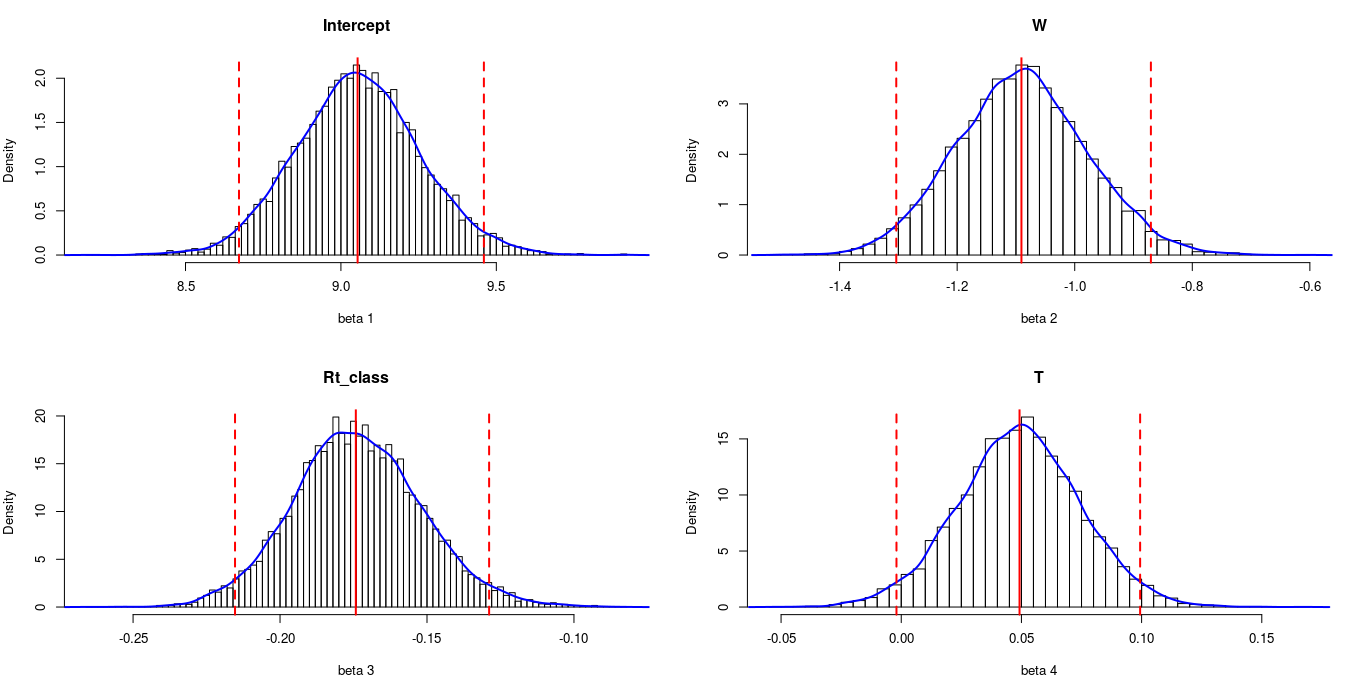
\includegraphics[width=120 mm]{pictures/negbin_single_r_beta.png}
	\caption{Distribution of the $\boldsymbol{\beta}$ regression parameters}
	\label{fig:nb_beta}
\end{figure}
Results of sampled $Y_t$ in correspondence to the 42 days under study are deeply different from the Poisson likelihood model. 90$\%$ credibility intervals are much larger, and the overall behaviour is caught. But the intervals widths are quite too large for real applications of the model, since the uncertainty described by the model determines too imprecise estimates. Here we show the situation:
\begin{figure}[H]
	\centering
	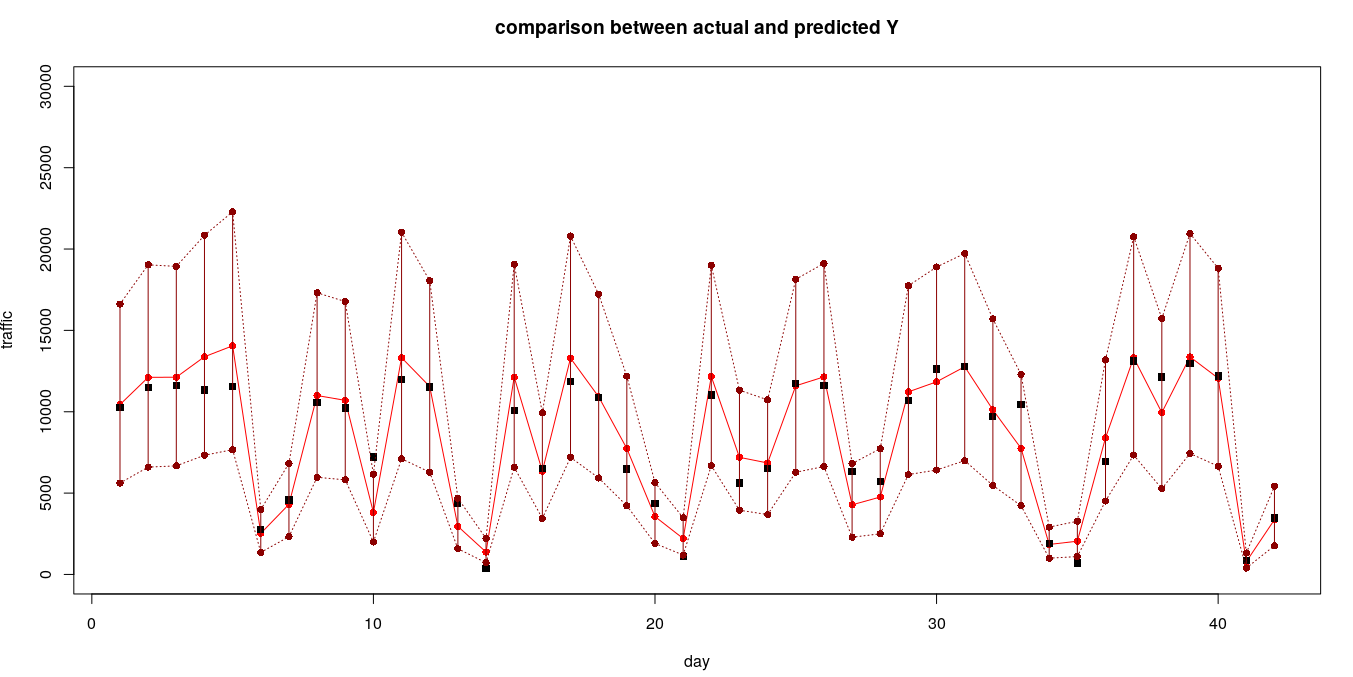
\includegraphics[width=120 mm]{pictures/negbin_single_r_pred.png}
	\caption{Sampled $Y_t$ for the 42 days, compared with the real data}
	\label{fig:nb_pred}
\end{figure}
We wondered if the highly different behaviour between weekends and weekdays could be better explained by introducing dispersion parameters $r$ specific for the two groups of days. On the other hand, we still assume the group effect on the mean of the distribution is only related to a global term: we suppose it does not affect rain and temperature influence on the response. The model proposed is a modification of the previous Negative Binomial likelihood:
\begin{model} Loglinear GLMM with Negative Binomial likelihood (2)\\
	\begin{equation*}
	\begin{aligned}
	&\textsc{Model}\\
	&Y_{tj}  |  p_{tj},r_j \overset{\independent}{\sim} NegBin(p_{tj},r_j), \ j = 1 (wkdays), 2 (wkends)\\
	&p_{tj} = \frac{r_j}{r_j+\mu_{tj}}\\
	&\log{\mu_{tj}} = \beta_1 + \beta_2R_{t} + \beta_3T_{t} + \theta_j\\
	&\\
	&\\
	\end{aligned}
	\qquad \qquad
	\begin{aligned}[c]
	&\textsc{Priors}\\
	&\beta_i | \tau_i \sim \mathcal{N}(0, \tau_i) \ i = 1,2,3\\
	&\tau_i \overset{\independent}{\sim} Gamma(2,10) \\
	&\theta_j | \tilde{\tau}_j \sim \mathcal{N}(0, \tilde{\tau}_j) \ j = 1,2\\
	&\tilde{\tau}_j \overset{\independent}{\sim} Gamma(2,10)\\
	&r_j \overset{\independent}{\sim}\mathcal{U}(0,50) \ j = 1,2
	\end{aligned}
\end{equation*}
	\end{model}
	We tried to implement the proposed model on Jags, but the chain was really badly simulated, as autocorrelation plots and stationarity were not acceptable, not even after long-time simulations. Therefore, we implemented the same model on Stan, which uses the alternative formulation with $\mu$ and $r$, and the diagnostic on the chain is definitely acceptable. The 90$\%$ credibility intervals of the corresponding 42 days prediction are shown in the following picture:
	\begin{figure}[H]
		\centering
		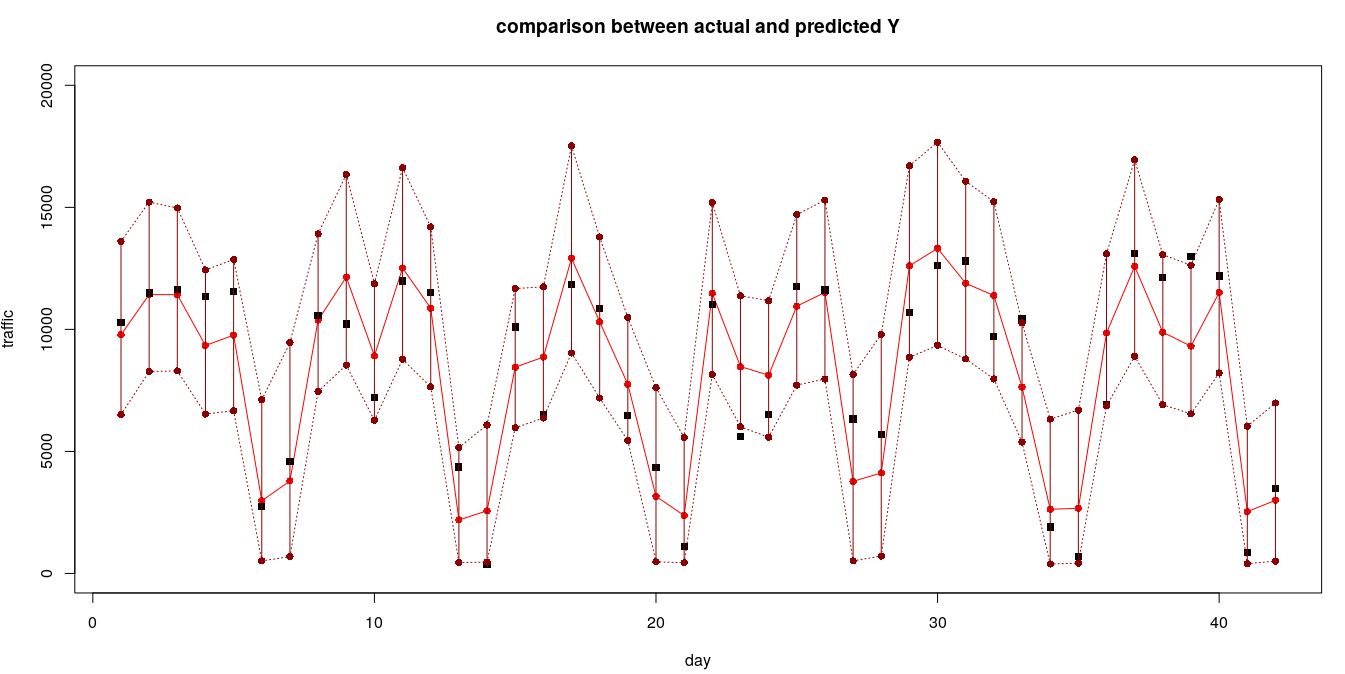
\includegraphics[width=160 mm]{pictures/negbin_double_r_pred.png}
		\caption{Sampled $Y_t$ for the 42 days, compared with the real data}
		\label{fig:nb_d_pred}
	\end{figure}
	This model seems to catch the overall phenomenon features, and the width of those intervals is shorter than the original Negative Binomial likelihood model. Only 4 data fall outside the associated intervals. However, the variance of our prediction is still quite high, so we wished to propose an even more suitable model for the problem.


\section{Bayesian Structural Time Series}
As a second operative approach, we tried to implement a Bayesian Structural Time Series model (BSTS). We can think this method as the Bayesian counterpart of the frequentis ARIMA representation: even though it does not rely on differencing, lags and moving averages, it makes possible to see historical data as the superposition of multiple effects, each one with its own meaning and interpretation. Moreover, the modularity of the BSTS approach, joint with the probability driven Bayesian model selection, makes it easier to quantify the posterior uncertainty of the individual components, perform variable
selection during model training, thus preventing overfitting, and also incorporate prior beliefs, possibly coming from time consistent, older data. 

\subsection{Introduction to BSTS}
Structural time series are basically state space models for historical data. In this subsection we will try to give a brief, but exhaustive, introduction to the topic stressing in particular the advantages deriving from the Bayesian approach, for a more complete and detailed description please refer to SV13 and JRN18 in bibliography.\\
\\
We can think a state space model as a couple of stochastic equations fed by independent noises and an initial condition:
\begin{equation}
\mathbf{y}_t = \mathbf{Z}_t \boldsymbol{\alpha}_t + \boldsymbol{\epsilon}_t,\quad \boldsymbol{\epsilon}_t \overset{\independent}{\sim} \mathcal{N}_m(0, \boldsymbol{\Sigma}_t),
\end{equation}
\begin{equation}
\boldsymbol{\alpha}_{t+1} = \mathbf{T}_t \boldsymbol{\alpha}_t + \mathbf{R}_t \boldsymbol{\eta}_t,\quad \boldsymbol{\eta}_t \overset{\independent}{\sim} \mathcal{N}_q(0, \mathbf{Q}_t),
\end{equation}
\begin{equation}
\boldsymbol{\alpha}_0 \sim \mathcal{N}_d(\boldsymbol{\mu}_0, \boldsymbol{\Sigma}_0)
\end{equation}
Borrowing the nomenclature from automatic control theory, the first relationship is called the observation equation, since it defines the $ \mathbb{R}^m$ vector of the observations at current time $ \mathbf{y}_t $ from the linear transformation $ \mathbf{Z}_t $ of a $ \mathbb{R}^d $ vector of the unobserved (and a priori fictitious) current latent states $ \boldsymbol{\alpha}_t $. The second identity is often known as transition equation, since it specifies latent states stochastic dynamics over time, or state equation. Within this context, $ d $ will be the overall number of latent states for all entries in $\mathbf{y}_t$ and model matrices $ \mathbf{Z}_t,\ \mathbf{T}_t,\ \mathbf{R}_t $ are made of known and unknown time varying parameters: $ \mathbf{Z}_t $ is the $ d \times m $ output matrix, $ \mathbf{T}_t $ is a $ d \times d $ transition matrix, and $ \mathbf{R}_t $ is a $ d \times q $ control matrix. $ \mathbb{R}^m $ vector $\boldsymbol{\epsilon}_t$ denotes observation errors with a $ m \times m $ variance matrix $ \boldsymbol{\Sigma}_t $, while $ \boldsymbol{\eta}_t $ is the $ q $-dimensional system error distributed with zero mean and a $ q \times q $ full rank state diffusion matrix $ \mathbf{Q}_t $, where $ q\leq d $. Finally the state is endowed with suitable random initial conditions.\\

There are two main advantages in the use of structural time series constructed in terms of components: first, each state variable can be analyzed both singularly or coupled together with the other effects, since addition of a new variable block is translated into a simple sum in terms of equations. This keeps the model representation elementary and enables evaluation through a Bayesian posterior probability approach. Moreover, provided state variables being added with criterion, state models can purposely give a meaningful interpretation for many building blocks of the scheme. As an example, just recall that in most ARIMA models the series is derived as the sum of a trend, the seasonality, maybe a local cycle and regression components, elicited through differentiation and use of moving averages. The state space counterpart of this, i.e. a quite flexible baseline for many STS models, can be written as:
\begin{equation}
\mathbf{y}_t = \boldsymbol{\mu}_t + \boldsymbol{\gamma}_t + \boldsymbol{\nu}_t + \boldsymbol{\beta}^T \mathbf{z}_t + \boldsymbol{\epsilon}_t
,\quad \boldsymbol{\epsilon}_t\overset{\independent}{\sim} \mathcal{N}_m(0, \boldsymbol{\Sigma}_t)
\end{equation}
where the summands are respectively trend, seasonality, cyclical component, regression and observation error. In the state space representation of before, $ \boldsymbol{\alpha}_t $ would be the vector containing these terms, $ \boldsymbol{\alpha}_t = [\boldsymbol{\mu}_t, \boldsymbol{\gamma}_t, \boldsymbol{\nu}_t, \mathbf{z}_t] $. However the model can undergo various simplifcations: often, for the sake of computation, $ \boldsymbol{\Sigma}_t=\boldsymbol{\Sigma}\ \forall t \in \{1:T\} $ is a constant positive definite matrix. Conversely, it can be also complicated as much as possible, for instance the regression summand might be made dynamic.

\subsection{Proposed global models}
In this subsection we will provide a brief overview of the main global models considered in our work, stating and commenting where necessary each one of them, discussing the results in light of a Bayesian setting and finally comparing the different outputs. Let's start from the one that will represent the benchmark for any further variation.

\subsubsection{Standard with autoregression}
This model is a compendium of all the ingredients peculiar of standard BSTS structures discussed in the previous subsection. Within this framework, it is possible to represent the output as sum of a locally linear trend $ \mu $ (depending on $ \delta $), a period $ \gamma $, a 1-step $ \alpha $-autoregression $ \rho $ and a linear regression term $ \boldsymbol{\beta} $ on $ \mathbf{z}$ suitably selected covariates. The state is made of the aforementioned quantities and evolves fed by four independent noises (plus the noise in output equation). The scale of these five quantities is given in terms of their precisions, for which is set an hyperprior with a Gamma distribution and fixed hyperparameters. Also the initial conditions are formulated in coherent form, depending on fixed hyperparameters and being independent from the other terms. Finally an hyperprior can be fixed for the regression coefficients and the autoregression factor as independent normals. Just a remark concerning  notation: $ \tau $s are precisions, gaussians are written in terms of precisions instead of variances, and $ hpm $ stays for hyperparameters.\\
\\
Unfortunately, the dynamic behaviour of this model is unstable under uninformative prior selection. Two were the main issues destablizing the MCMC runs: having initial conditions with fixed precision (i.e. in general too precise w.r.t. the actual uncertainty of the subsequent time slots), and the uneven distribution of variability between state and output errors. In order to give homogeneity to the credibility of the initial conditions, we decided to set them, not as hyperparameters, but random, equal to the corresponding precisions of their dynamic equivalents. Moreover, it proved necessary to substitute the gamma distributions for the precisions with uniforms in intervals of suitable magnitude. The root of this decision is given by computational problems. If left free to evolve MCMC runs of JAGS tend to collect all the amount of uncertainty on the output error, leaving costant in time both trend and period. This erratic coagulation of the uncertanty can be prevented forcing the state errors to keep a suitable magnitude order (i.e. fixing a min/max for them). In general this produces better results and eventually the stability is preserved.


\begin{model} Corrected standard BSTS with autoregrssion
	\begin{equation*}
	\begin{aligned}
	&\textsc{Model}\\
	&Y_t = \mu_t + \gamma_t + \rho_t + \boldsymbol{\beta}^T\mathbf{z}_t + \tau_\epsilon^{-\frac{1}{2}}\tilde{\epsilon}_t\\
	&\mu_t = \mu_{t-1} + \delta_{t-1} +\tau_\eta^{-\frac{1}{2}}\tilde{\eta}_t\\
	&\delta_t = \delta_{t-1} + \tau_v^{-\frac{1}{2}}\tilde{v}_t\\
	&\gamma_t = \sum_{i=1}^{S-1}\gamma_{t+i-S} + \tau_w^{-\frac{1}{2}}\tilde{w}_t\\
	&\rho_t = \alpha\rho_{t-1} + \tau_u^{-\frac{1}{2}}\tilde{u}_t\\
	&\tilde{\epsilon}_t, \tilde{\eta}_t, \tilde{v}_t, \tilde{w}_t, \tilde{u}_t \overset{iid}{\sim} \mathcal{N}(0,1)\\
	\\
	&\textsc{Initial Conditions}\\
	&\mu_0 \sim \mathcal{N}(m, \tau_\eta)\quad \quad \quad \quad \quad\  m\ \ hpm\\
	&\delta_0 \sim \mathcal{N}(d, \tau_v)\quad \quad \quad \quad \quad \quad d\ \ \ hpm\\
	&\boldsymbol{\gamma}_{0:(2-S)} \sim \mathcal{N}_{S-1}(\mathbf{g}, \tau_w\mathbf{I})\quad\ \ \mathbf{g}\ \ hpm\\
	&\rho_0 \sim \mathcal{N}(r, \tau_u)\quad \quad \quad \quad \quad \quad \ r\ \ hpm\\
	\\
\end{aligned}
\qquad \qquad
\begin{aligned}[c]
	&\textsc{Priors}\\
	&\boldsymbol{\beta} \sim \mathcal{N}_p(\mathbf{0}, \tau_b \mathbf{I})\ \ \quad \quad \quad \quad \quad \tau_b\ \quad \ hpm\\
	&\alpha \sim \mathcal{N}(a, \tau_a) \ \quad \quad \quad \quad \quad \quad a, \tau_a\ \ hpm\\
	&\tau_\epsilon \sim Unif(a_\epsilon, b_\epsilon)\quad\quad\ \quad \quad a_\epsilon, b_\epsilon\ \ hpm\\
	&\tau_\eta \sim Unif(a_\eta, b_\eta)\quad\quad\quad \quad a_\eta, b_\eta\ \ hpm\\
	&\tau_v \sim Unif(a_v, b_v)\quad\quad\quad \quad a_v, b_v\ \ hpm\\
	&\tau_w\sim Unif(a_w, b_w)\quad\quad\quad\ a_w, b_w\ \ hpm\\
	&\tau_u \sim Unif(a_u, b_u)\quad\quad\quad\quad a_u, b_u\ \ hpm\\
	&\\
	&\\
	&\\
	&\textsc{Independence}\\
	&\{\tilde{\epsilon}_t, \tilde{\eta}_t, \tilde{u}_t, \tilde{w}_t, \tilde{v}_t, \mu_0, \delta_0, \boldsymbol{\gamma}_{0:(-S+2)}, \rho_0,\\ &\boldsymbol{\beta}, \alpha, \tau_\epsilon, \tau_\eta, \tau_v, \tau_w, \tau_u\}\\ &family\ of \independent real\ random\ variables\\
	&\\
	&\\
\end{aligned}
\end{equation*}
\end{model}
\paragraph{Implementation}  The model has been implemented in bug language in order to be read by $ \texttt{rjags} $ package in R environment. Hyperparameters for precisions have been fixed in an uninformative way (using uniform distributions) or with extremely small precisions in case of gaussian density. All the values are detailed within this table:\\

\begin{table}[!htb]
	\begin{subtable}{.5\linewidth}
		\centering
\begin{tabular}{|c|c|c|c|c|c|}
	\hline
	& $ \tau_\epsilon $ & $ \tau_\eta $ &$  \tau_v $ & $ \tau_w $ & $ \tau_ u $\\
	\hline
	a &$  1\mathrm{e}{-7} $ & $  1\mathrm{e}{-5} $ &$  1\mathrm{e}{-5} $&$  1\mathrm{e}{-5} $&$  1\mathrm{e}{-5} $\\
	\hline
	b &$  1\mathrm{e}{-4} $ & $  1\mathrm{e}{-4} $ &$  1\mathrm{e}{-4} $&$  1\mathrm{e}{-4} $&$  1\mathrm{e}{-3} $\\
	\hline
\end{tabular} 
	\end{subtable}%
	\begin{subtable}{.5\linewidth}
		\centering
	\begin{tabular}{|c|c|c|c|c|}
		\hline
		& $ \tau_\alpha $ & $ \tau_\beta $ & $ r $ & $ d $\\
		\hline
		value &$  1\mathrm{e}{-5} $ & $  1\mathrm{e}{-5} $& 0 & 0\\
		\hline
	\end{tabular} 
	\end{subtable} 
\end{table}

For what concerns $ m $ and $ \mathbf{g} $, their value is assigned using the estimate provided by moving average and periodicity from the frequentist statistical tools discussed in the preliminary phase. This choice is made in order to set the initial conditions at a reasonable value, taking advantage of the conceptual link between STS periodicity and filtered priodicity, trend and moving average, as pointed out in the previous section. The regression $ \boldsymbol{\beta}^T\mathbf{z} $ part can be expressed as $ (\beta_1+\nu_1w)z_1 + (\beta_2+\nu_2w)z_2$, a mixed effect model of the kind $ \mathit{common\ value + group\ specific\ correction} $. $ w $ is an indicator function that takes either value $ 1 $, if the day is part of a weekend, or $ 0 $ else; $ z_1 $ and $ z_2 $ are respectively a scaled factor denoting the amount of rain forecasted for the day and the average daily temperature registered. These covariates are among the ones suggested by both the frequentists analyisis and the loglinear model selection. We will discuss their importance and role in the following paragraphs.

\paragraph{Diagnostics}
Let us discuss the godness of the chains produced by JAGS MCMC samples.
The following boxplots enlight about both the stability and the values assumed by the parameters. As we can see, after having run approximately 500000 samples with a thinning of 20 units in order to avoid high autocorrelation and 10000 units burnin, we have reached a good degree of stationarity. However, it appears quite clear that factor $ \alpha $ is not likely to be cosidered different form zero, since its distribution appears completely centered on that value, thus making the autoregressive part seem definitely useless. Different argument for terms $ \beta $ and their $ \nu $ corrections: on the opposite they have values quite strongly differing from 0. Note in particular that the first coefficient $ \beta_1 $, linked to the presence of rain, is negative, just as it was expected.  Let's now discuss the chain mixing of the Gibbs sampler's MCMC runs used by JAGS to draw posterior distributions. Results are quite similar in both cases, even when the thinning is selected at the smaller quantity. However if we want to see nice autocorrelation plots we need to reach at least the second value. As it can easily be deduced from the following pictures, autocorrelation plots are acceptable in all cases but on term $ \beta_2 $ which appears very autocorreleated, even though the final shape of the distribution seems to match pretty well that of a gaussian. Opposite behaviour for $ \alpha $ which has a completely uniform nature, testifying the lack of precision in this term estimation (luckily, note that this factor is so small to not influence very much the rest). Nonetheless, given the poor performances and weak worth, we will discuss the elimination of this factor in further developments.

\begin{figure}[H]
	\begin{subfigure}[H]{0.50\linewidth}
		\centering
		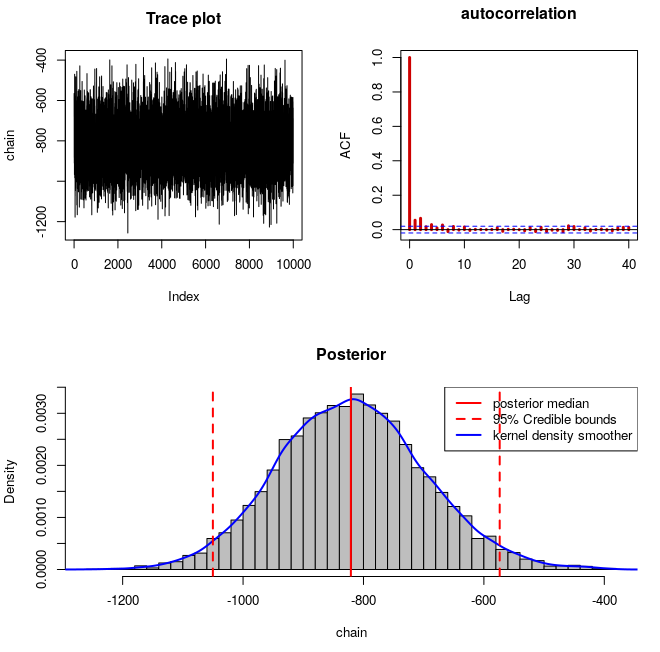
\includegraphics[width=50 mm]{pictures/beta_1.png}
		\caption{Diagnostics for $ \beta_1 $ samples}
		\label{fig:beta_1}
	\end{subfigure}
	\hfill
	\begin{subfigure}[H]{0.50\linewidth}
		\centering
		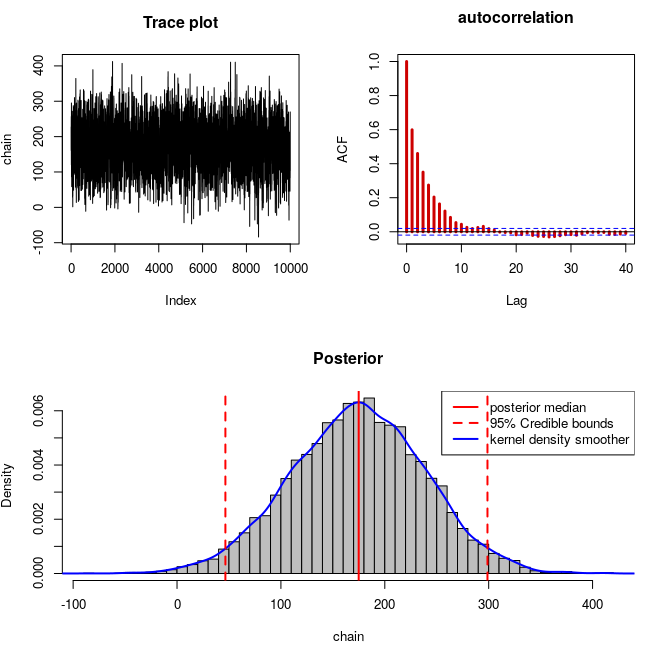
\includegraphics[width=50 mm]{pictures/beta_2.png}
		\caption{Diagnostics for $ \beta_2 $ samples}
		\label{fig:beta_2}
	\end{subfigure}%
\end{figure}

\paragraph{Results}
We  will now discuss in detail the results produced by this model, provided its validation from a diagnostic viewpoint. In particular we will focus on the structural capability of predicting the outcome of the time series, i.e. how close does our prediction come with respect to the actual observed data.

\begin{figure}[H]
		\centering
		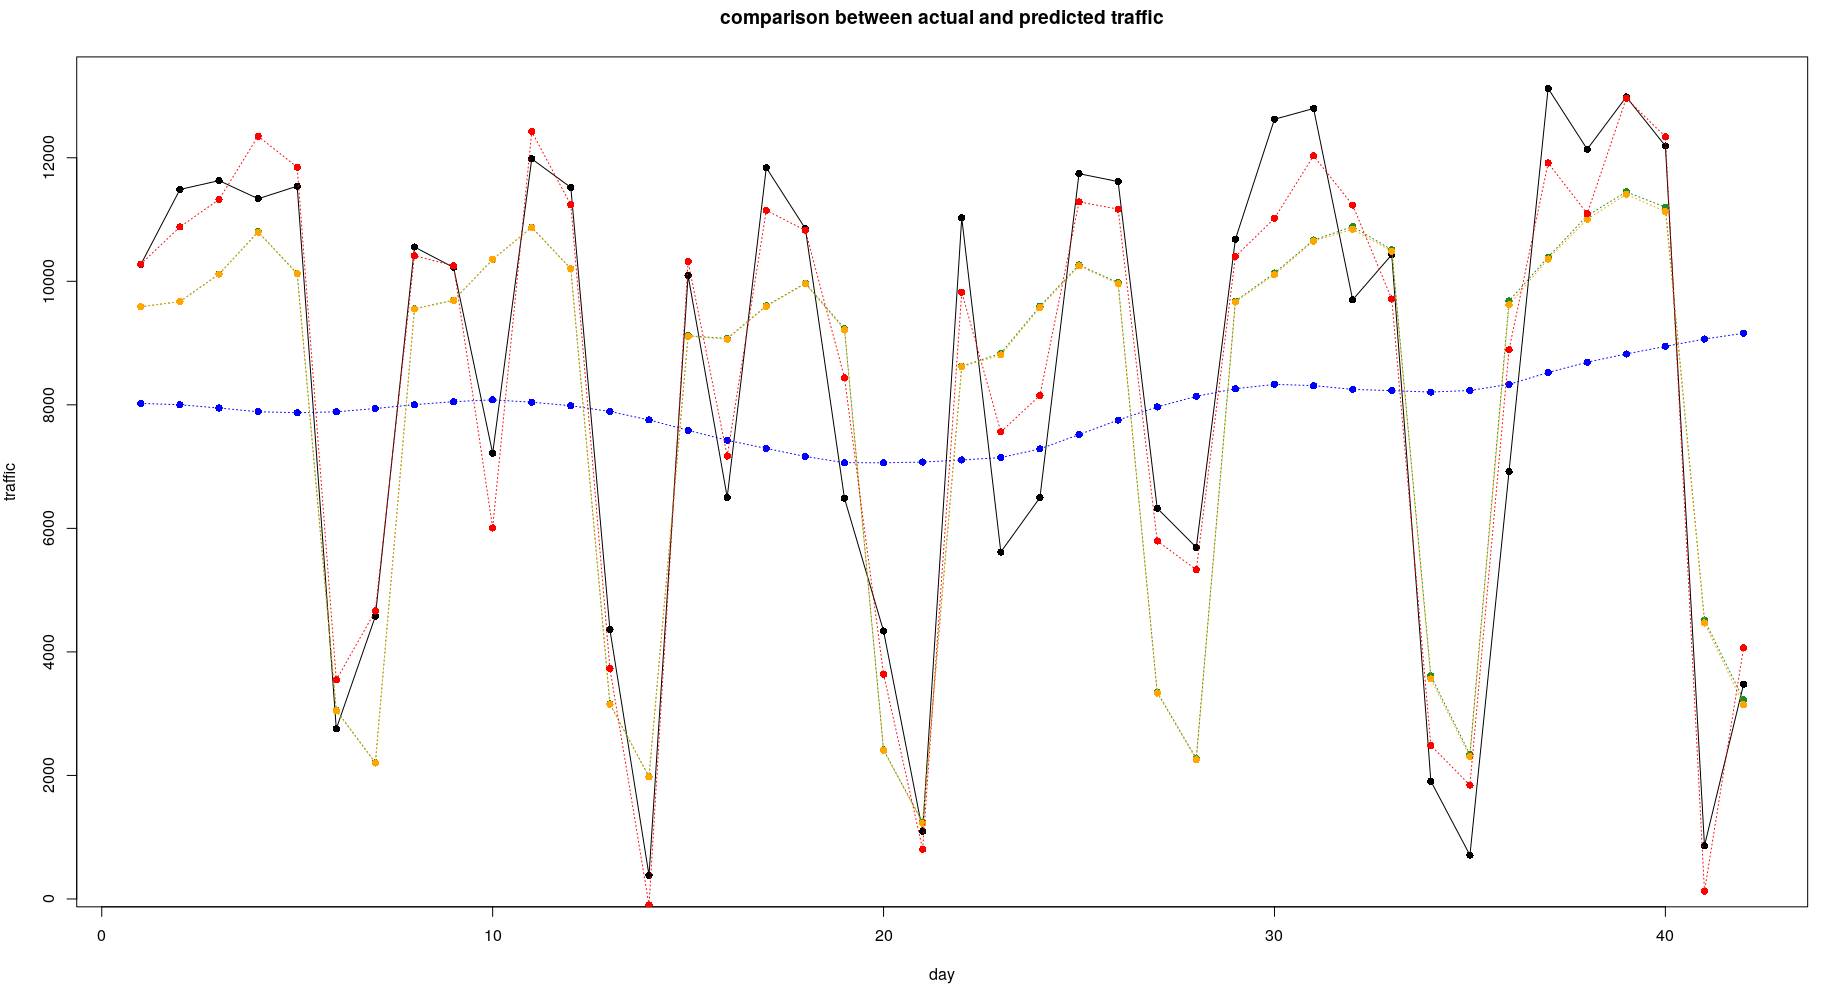
\includegraphics[width=150 mm]{pictures/m2_g1.png}
		\caption{Sum of trend (blue), periodicity (green), autoregression (yellow) and regression (red)}
		\label{fig:M2_p1}
	\end{figure}

In picture \ref{fig:M2_p1} it is possible to see the superposition of different components of the state and the prediction that can be deduced from them. It is evident that both trend and periodicity are perfectly in line with their abstract meaning and note that this fact is absolutely not trivial since the evolution of the MCMC is completely free and driven only by the rules constituting the model. In principle the final solution might had stabilized to values very far from the intuitve meaning that we gave to these terms of the state. Seeing our intuition being met is surely an indirect hint showing the model's ability to capture the essence of the process generating the data. Moreover the fact that the functions are slow varying may suggest us the avoidability of a robust method, that we will however try anyway for the sake of comparison. Coversely, just as pointed out during the diagnostics phase the action of the autoregression part seems irrelevant since the yellow and green line are almost cohincident.\\
\\
Fundamental is also the role of the regression component that, summed to aforementioned parts is able to capture quite well the shape of the original function. In particular the slope of some increments changes between pre and post addition of the regression to the model and mostly of the times this change meets what actully happens in the original profile. This can be considered a positive signal, since trend, periodicity and autoregression are good only to fix the mesocale form of the function, the local behaviour is very difficult to be captured by these terms. The fact that a strong positive correction is performed by the addition of the linear regression entails the presence of a strong local dependence. This fact is absolutely coherent with what is supposed to happen in reality since, very often, it is up to the climatic conditions to dictate the effective number of bikes moving on the network on a certain day. Note that the standard deviation of our predictive dstribution is approximately of 1000 trips. Moreover, almost all the times, data lie within the intervals suggested by the model.\\
\\
There is just a small portion (2-3 among 42) of data which are not captured well by the model and often belong to days with a strong - but short - rainy phenomena, for which the scale factor is too vague in order to take into account sharp variations in the same day and only one possibility can be accepted (the day have to be classified either as sunny or rainy according to the information at our disposal, hence making impossibe a more detailed level of prediction). For this reason, as a final comment, we can consider the model designed in this paragraph a good staring point from which to try some improvements or simplifications. We will mainly focus on three variants: without temperature as a covariate, without autoregression and the robust version. Finally let us conclude this pragraph with the plot of a possible prediction of the future done by the chain, using the predictor which minimizes quadratic loss (expected value) and reporting 90\% confidence bands. A short remark, given the strong stability of the prediction we might expect not to be necessary a robut version of it. We will clarify this point in a didicated section where comparisons will be made from a predictive viewpoint.

\begin{figure}[H]
	\centering
	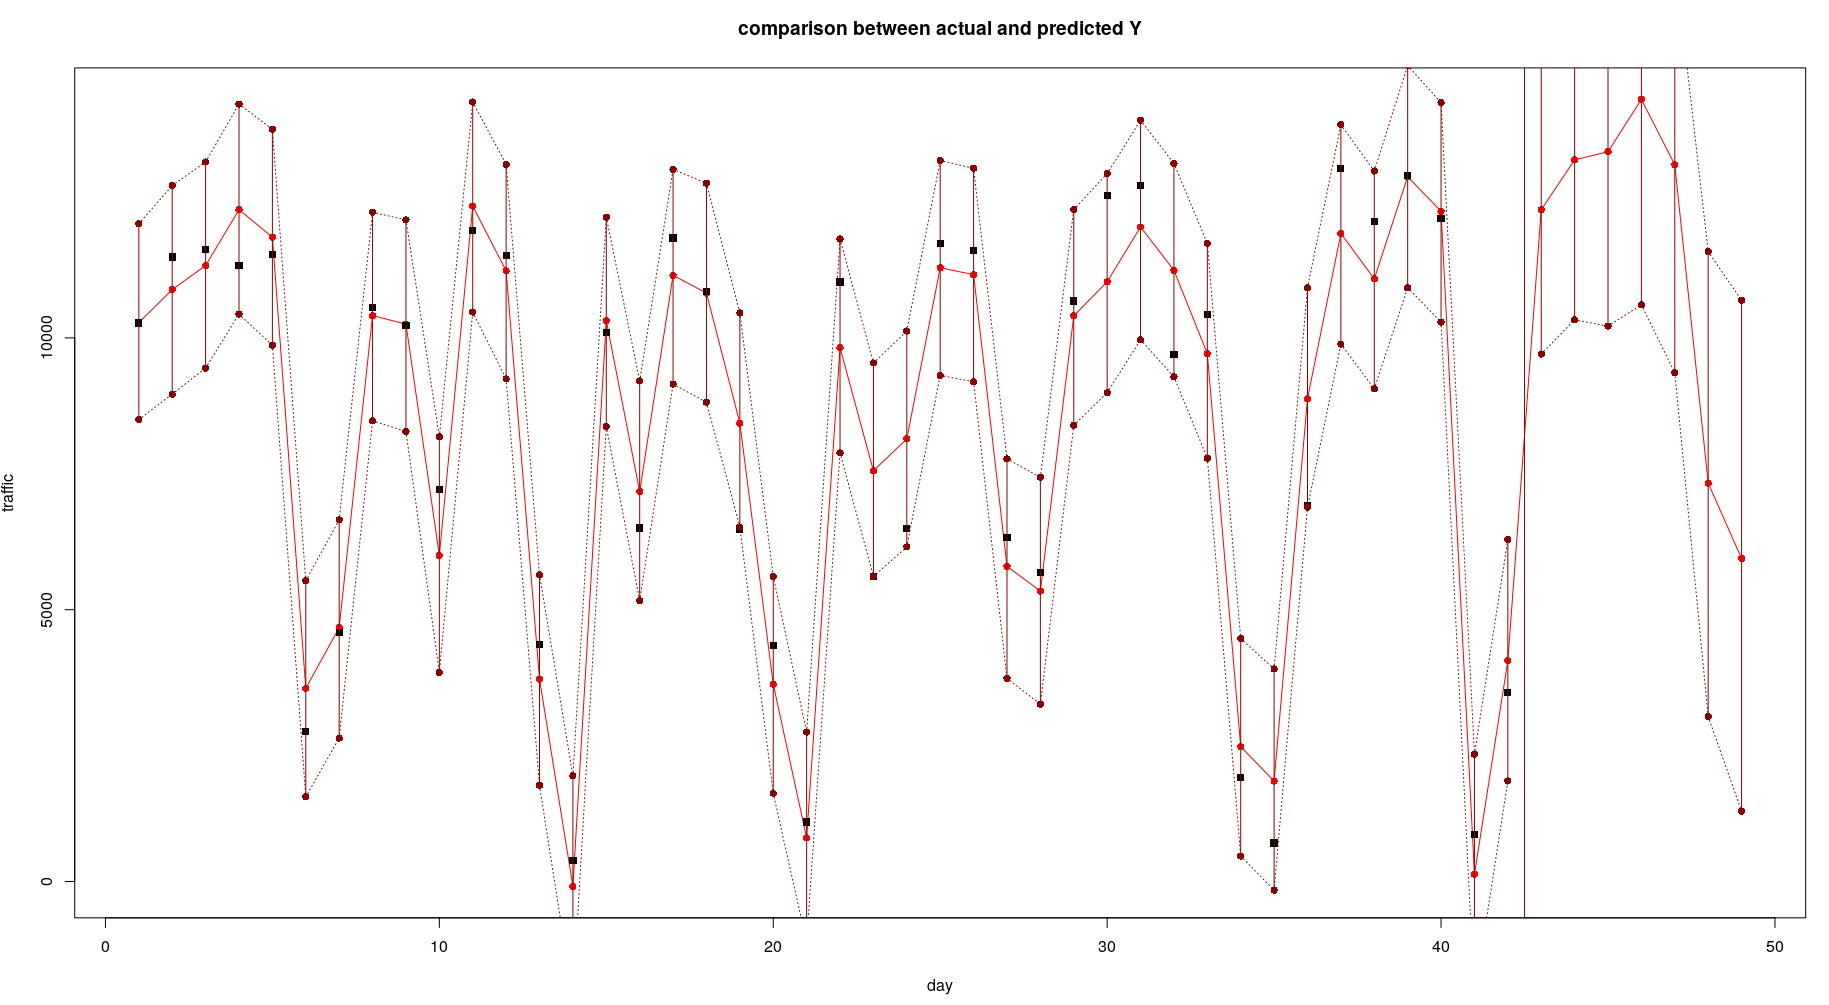
\includegraphics[width=150 mm]{pictures/m1_future.png}
	\caption{Present and future prediction according to the model}
	\label{fig:M1_future}
\end{figure}

\subsubsection{Standard with autoregression, without temperature}
Given the relative importance represented by temperature in our models, often resulting in a mere quite uniform vertical translation of the whole function, we can take into consideration its elimination from the set of regressors and a possible incorporation of its non-negative action in the trend. We will see what happens to the previous model under these modifications and discuss their worth. Just keep into account that the only difference with the previous model lies in term $ \boldsymbol{\beta}^T\mathbf{z} $ now reduced from $ (\beta_1+\nu_1w)z_1 + (\beta_2+\nu_2w)z_2$ to $(\beta+\nu w)z_1$.


\paragraph{Results} The predicted time series appears qualitatively slightly more inaccurate (higher variability implies increased size of the credibility intervals). Note also that the trend has a more oscillating behaviour, this might indicate that the effect of temperature has been absorbed by this term, destibilizing it a bit. Bayesian residuals and predictive p-values are too similar with the previous case to be a direct matter of comparison. Also the estimated number outliers is always oscillating betwen two and three. Thus, it's better to entrust this role to other more effective strategies, like automatic evaluation procedures. We will discuss the results together with that of the robust model in the next paragraph.

\subsubsection{Robust standard with autoregression model}
In order to better evaluate the worth of our original model it may seem wise to compare it with a more robust version, where the dependencies are fixed in way that each term of the trend and slope is made dependent not only on its past value (i.e current time), but also on some analogue days in the past: the idea is to use operator $ \mathcal{L}_t(\cdot) = \frac{1}{2}(\cdot)_{t-1} + \frac{1}{3}(\cdot)_{t-S} +\frac{1}{6}(\cdot)_{t-2S} $. .
\begin{figure}[H]
	\centering
	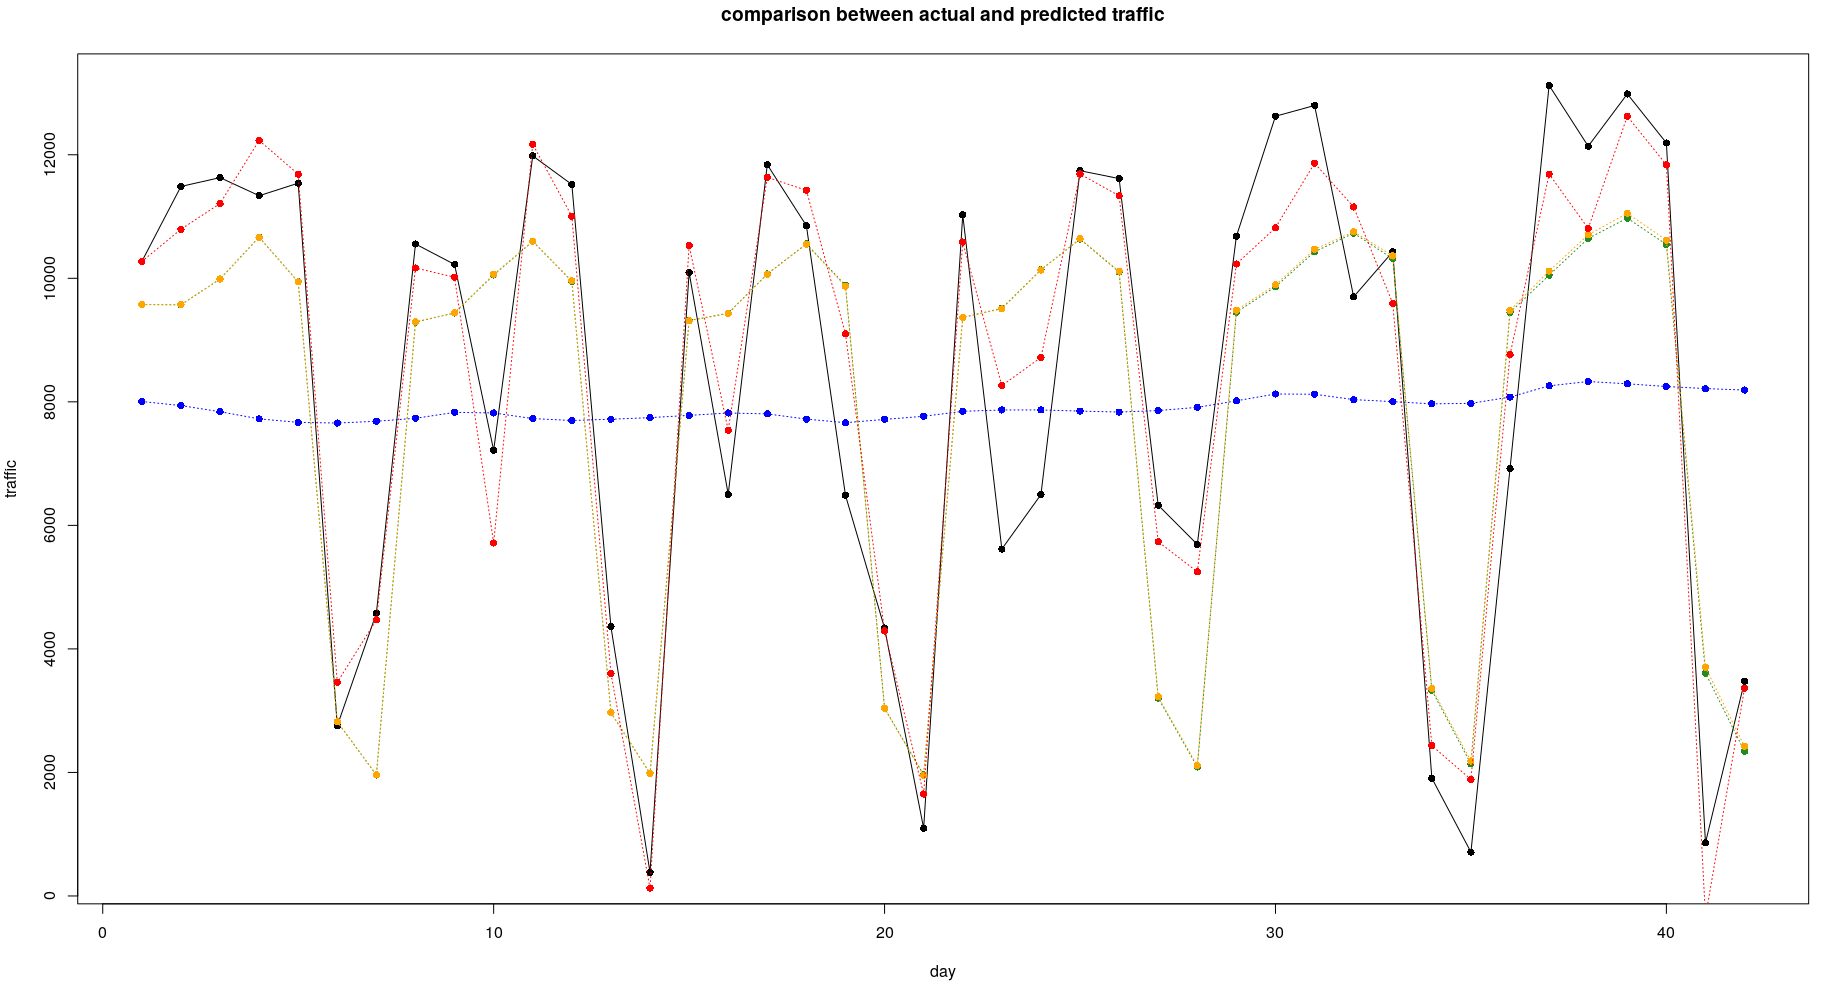
\includegraphics[width=150 mm]{pictures/m4_p1.png}
	\caption{Cumulative action of trend (blue), periodicity (green), autoregression (yellow) and regression (red) in robust model}
	\label{fig:M4_p1}
\end{figure}
\paragraph{Results}
It is possible to show that boxplots regarding this section are approximately similar to the ones without the presence of temperature within the regressors, i.e. stable, but with a lower precision on the output error. As always this might be considered a factor suggesting a worsening in the partition of uncertainty between state and output. But differently from the previous case, where the state is forced to oscillate too much for a lack of accuracy at local level, here the variation is due to an increased inability of the state (and in particular the trend-slope) to fit the fluctuations of the data. Indeed, as it can also be shown by the following picture there is a high risk of trend oversmoothing.
It has to be remarked that even though the number of outliers is unchanged from the previous models, the three "historical" outliers of the problem are even more uncapturated than in the previous cases. We are now going to discuss wich model among standard, robust and without temperature should be considered the best according to the criteria discussed in the previous section. Using the mean normalized residuals in time as an evaluation criterion the values are not varying too much, the smallest is reached for the standard model, hence it should be considered the best, at least according to this criterion. As for mean tail probabilities, the version without temperature seems slightly more accurate than the others (on average), however the difference with the standard is so close that we can still continue to prefer it, especially in light of the shape of the trend interpretation discussed before. Finally, since also the $ elpd_{loo} $ takes its maximum in correspondence of the standard model, so that we can agree about this being considered the best among the ones seen so far. As a further step, we will immediately ponder the elimination  of the autoregresive part, that we have seen being more a badly playing figurant rather than a protagonist.

\begin{table}[!htb]
		\centering
		\begin{tabular}{|c|c|c|c|}
			\hline
			& standard & no temperature & robust \\
			\hline
			Mean standardized residuals &$  0.5809041 $ & $  0.6066627 $ &$  0.6031869 $\\
			\hline
			Mean tail probabilities &$ 0.2979543 $ & $  0.298591 $ &$  0.2908414 $\\
			\hline
			$ elpd_{loo} $ &$ -362.6 $ & $  -365.4 $ &$  -364.1 $\\
			\hline
		\end{tabular}
\end{table}
 
 \subsection{Global model with time zones}
 The last BSTS model we want to present is a variation of the previous cases defined to capture the difference in time zones across various days. Note that the structures discussed so far have always had as main goal that of making inference about the overall amount of bikes running on the network in a certain day. The aim of this section is different. In the data preprocessing we got the chance to subdivide the overall traffic in four meaningful standard time zones: morning (6 a.m - 9 a.m), midday (10 a.m. - 3 p.m.), late afternoon (4 p.m. - 7 p.m.) and night (8 p.m. - 1 a.m). We are now going to make predictions dividing the flow in these groups, trying to fit an evolution of standard BSTS model without autoregression which suits well these separations.
 As a main modification, we will have to introduce a way to capture the flow of traffic within a certain day. This can be done in a rather easy way, exploiting the modularity of BSTS approach. As mentiond in the introduction, BSTS is able to support multiple periodicities within the same framework and this is exactly what can be turned in a strong advantage. Indeed, adding a second inner cycle covering a whole day, we can get the superposition of two loops and hence derive the output as sum of locally linear trend, a regression factor and these two effects. Note that in the following $ t $ will denote the day (ranging from 1 to 42) while $ h $ is the time fraction in $ 1:4=F $. $ S=7 $, as always, is the number of days in a week.
 
 \begin{model} Corrected standard BSTS with time zones
 	\begin{equation*}
 	\begin{aligned}
 	&\textsc{Model}\\
 	&Y_{F(t-1)+h} = \\&\quad\quad
 	\mu_{t} + \gamma_{t} + \chi_{F(t-1)+h} + \boldsymbol{\beta}^T\mathbf{z}_{th} + \tau_\epsilon^{-\frac{1}{2}}\tilde{\epsilon}_{F(t-1)+h}\\
 	&\mu_t = \mu_{t-1} + \delta_{t-1} +\tau_\eta^{-\frac{1}{2}}\tilde{\eta}_t\\
 	&\delta_t = \delta_{t-1} + \tau_v^{-\frac{1}{2}}\tilde{v}_t\\
 	&\gamma_t = \sum_{i=1}^{S-1}\gamma_{t+i-S} + \tau_w^{-\frac{1}{2}}\tilde{w}_t\\
 	&\chi_{F(t-1)+h} = \sum_{j=1}^{F-1}\chi_{F(t-1)+h+j-F} + \tau_u^{-\frac{1}{2}}\tilde{u}_{F(t-1)+h}\\
 	&\tilde{\epsilon}_{F(t-1)+h}, \tilde{\eta}_t, \tilde{v}_t, \tilde{w}_t, \tilde{u}_{F(t-1)+h} \overset{iid}{\sim} \mathcal{N}(0,1)\\
 	\\
 	&\textsc{Initial Conditions}\\
 	&\mu_0 \sim \mathcal{N}(m, \tau_\eta)\quad \quad \quad \quad \quad\  m\ \ hpm\\
 	&\delta_0 \sim \mathcal{N}(d, \tau_v)\quad \quad \quad \quad \quad \quad d\ \ \ hpm\\
 	&\boldsymbol{\gamma}_{0:(2-S)} \sim \mathcal{N}_{S-1}(\mathbf{g}, \tau_w\mathbf{I})\quad\ \ \mathbf{g}\ \ hpm\\
 	&\boldsymbol{\chi}_{0:(2-F)} \sim \mathcal{N}_{F-1}(\mathbf{c}, \tau_u\mathbf{I})\quad\ \  \mathbf{c}\ \ hpm\\
 	\\
 	\end{aligned}
 	\qquad \qquad
 	\begin{aligned}[c]
 	&\textsc{Priors}\\
 	&\boldsymbol{\beta} \sim \mathcal{N}_p(\mathbf{0}, \tau_b \mathbf{I})\ \ \quad \quad \quad \quad \quad \tau_b\ \quad \ hpm\\
 	&\tau_\epsilon \sim Unif(a_\epsilon, b_\epsilon)\quad\quad\ \quad \quad a_\epsilon, b_\epsilon\ \ hpm\\
 	&\tau_\eta \sim Unif(a_\eta, b_\eta)\quad\quad\quad \quad a_\eta, b_\eta\ \ hpm\\
 	&\tau_v \sim Unif(a_v, b_v)\quad\quad\quad \quad a_v, b_v\ \ hpm\\
 	&\tau_w\sim Unif(a_w, b_w)\quad\quad\quad\ a_w, b_w\ \ hpm\\
 	&\tau_u\sim Unif(a_u, b_u)\quad\quad\quad\ \ a_u, b_u\ \ hpm\\
 	&\\
 	&\\
 	&\\
 	&\\
 	&\\
 	&\\
 	&\textsc{Independence}\\
 	&\{\tilde{\epsilon}_t, \tilde{\eta}_t, \tilde{w}_t, \tilde{v}_t, \mu_0, \delta_0, \boldsymbol{\gamma}_{0:(-S+2)}, \boldsymbol{\chi}_{0:(2-F)},\\&\boldsymbol{\beta}, \tau_\epsilon, \tau_\eta, \tau_v, \tau_w, \tau_u \}\\ &family\ of \independent real\ random\ variables\\
 	&\\
 	&\\
 	\end{aligned}
 	\end{equation*}
 \end{model}

\paragraph{Hyperpameters}
The hyperparameters used in this model are substantially equivalent to the ones seen in the previous subsections, with some slight variations, starting from the regression part. Encouraged by the results discussed in the full-day case we kept track of both temperature and rain. Unfortunately, as already remarked above, the data at our disposal have a daily accuracy hence we were not able to get precise estimates for the single time slots using simply this information. Nonetheless the regression proved to be a fundamental factor also in this case. Concerning the structure of $ \boldsymbol{\beta}^T\mathbf{z} $, we opted for the following rule: $ \boldsymbol{\beta}^T\mathbf{z} = (\beta_1+\nu_1\mathbb{I}_{weekend}(t)+\xi_h)\cdot z_1(F(t-1)+h) + (\beta_2+\nu_2\mathbb{I}_{weekend}(t))\cdot z_2(F(t-1)+h)$, where $ \boldsymbol{\beta} $ is the common baseline for all days, $ \boldsymbol{\nu} $ is the particular action of weekends, and $ \boldsymbol{\xi} $ is the correction to the effect created by of rain given by the time slot (namely the correction will be less strong in hours where the traffic is weaker). Moreover $ \boldsymbol{\beta},\boldsymbol{\nu},\boldsymbol{\xi}\independent\mathcal{N}(0,\tau_*) $ and we use uninformative priors, indeed:

\begin{table}[!htb]
	\begin{subtable}{.5\linewidth}
		\centering
		\begin{tabular}{|c|c|c|c|c|c|}
			\hline
			& $ \tau_\epsilon $ & $ \tau_\eta $ &$  \tau_v $ & $ \tau_w $ & $ \tau_ u $\\
			\hline
			a &$  1\mathrm{e}{-7} $ & $  1\mathrm{e}{-5} $ &$  1\mathrm{e}{-5} $&$  1\mathrm{e}{-5} $&$  1\mathrm{e}{-5} $\\
			\hline
			b &$  1\mathrm{e}{-4} $ & $  1\mathrm{e}{-4} $ &$  1\mathrm{e}{-4} $&$  1\mathrm{e}{-4} $&$  1\mathrm{e}{-4} $\\
			\hline
		\end{tabular} 
	\end{subtable}%
	\begin{subtable}{.5\linewidth}
		\centering
		\begin{tabular}{|c|c|c|c|c|}
			\hline
			& $ \tau_\nu $ & $ \tau_\beta $ & $ \tau_\xi $ & $ d $\\
			\hline
			value &$  1\mathrm{e}{-5} $ & $  1\mathrm{e}{-5} $& $ 1\mathrm{e}{-5} $ & 0\\
			\hline
		\end{tabular} 
	\end{subtable} 
\end{table}

While $ \mu_0 $, $ \boldsymbol{\chi}_{0} $ and $ \boldsymbol{\gamma}_{0} $ are initialized using information coming form the frequentist stationarization. $ \mu_0 $ is the moving average divided by $ 4 $, same for the periodic component with respect to the moving period, while $ \chi $ follows as the difference in fluctuation averaged  along time slots (i.e. it is the average in time for each $ h $ of the difference between single $ y_{th} $ and moving average + period correspondig to that $ t $). As it can be deduced from results, the shapes of all the regression coefficents are definitely good: traceplots are fat enough and autocorrelation is kept under control, at least besides $\beta_2$ case which has been proved being erratic also in the previous subsections. Note in particular how number 0 dwells inside almost all the intervals, however it is evident that mostly of the cases hypotheses of the type $ coefficient=0 $ are very far from being acceptable. These results are a nasty consequence of the high uncertainty due to the lack of data. It is obvious that in a richer context, having much more data at our disposal, not only the distribution of these terms would be esimated with increased accuracy, but probably also the variability of parameters would be shrunk. 

\paragraph{Results}
Figure \ref{fig:time series} shows the results of the analysis: in black we have the real observations, in red - linked by another line - our best prediction according to the mean squared error (posterior mean of $ y $). As we can see the lines are pretty much smilar and show most of the differences in days where there are strong rainy phenomena centered in a few hours of the day, for which we can only guess daily information irrespectively of intensity and duration. Moreover, it should be noted the ability of the structure to capture both weekdays an weekends, as shown by the confidence bars with which is endowed the mean line. However, the most interesting fact is given by the capability, not only to catch the real observations within credibility intervals, but also to follow the behaviour among several hours of the day: i.e. the model does not only appear locally reliable, but most of the times is also capable of predicting the slope between two consecutive observations (i.e if in the next time zone values will be higher or lower than the present ones). This is fundamental for strategies of adaptive control that try to follow the daily dynamics of the process in order to correct $ in\ medias\ res $ the possible shortages which may happen in the net, at least from a global viewpoint.

\begin{figure}[H]
	\centering
	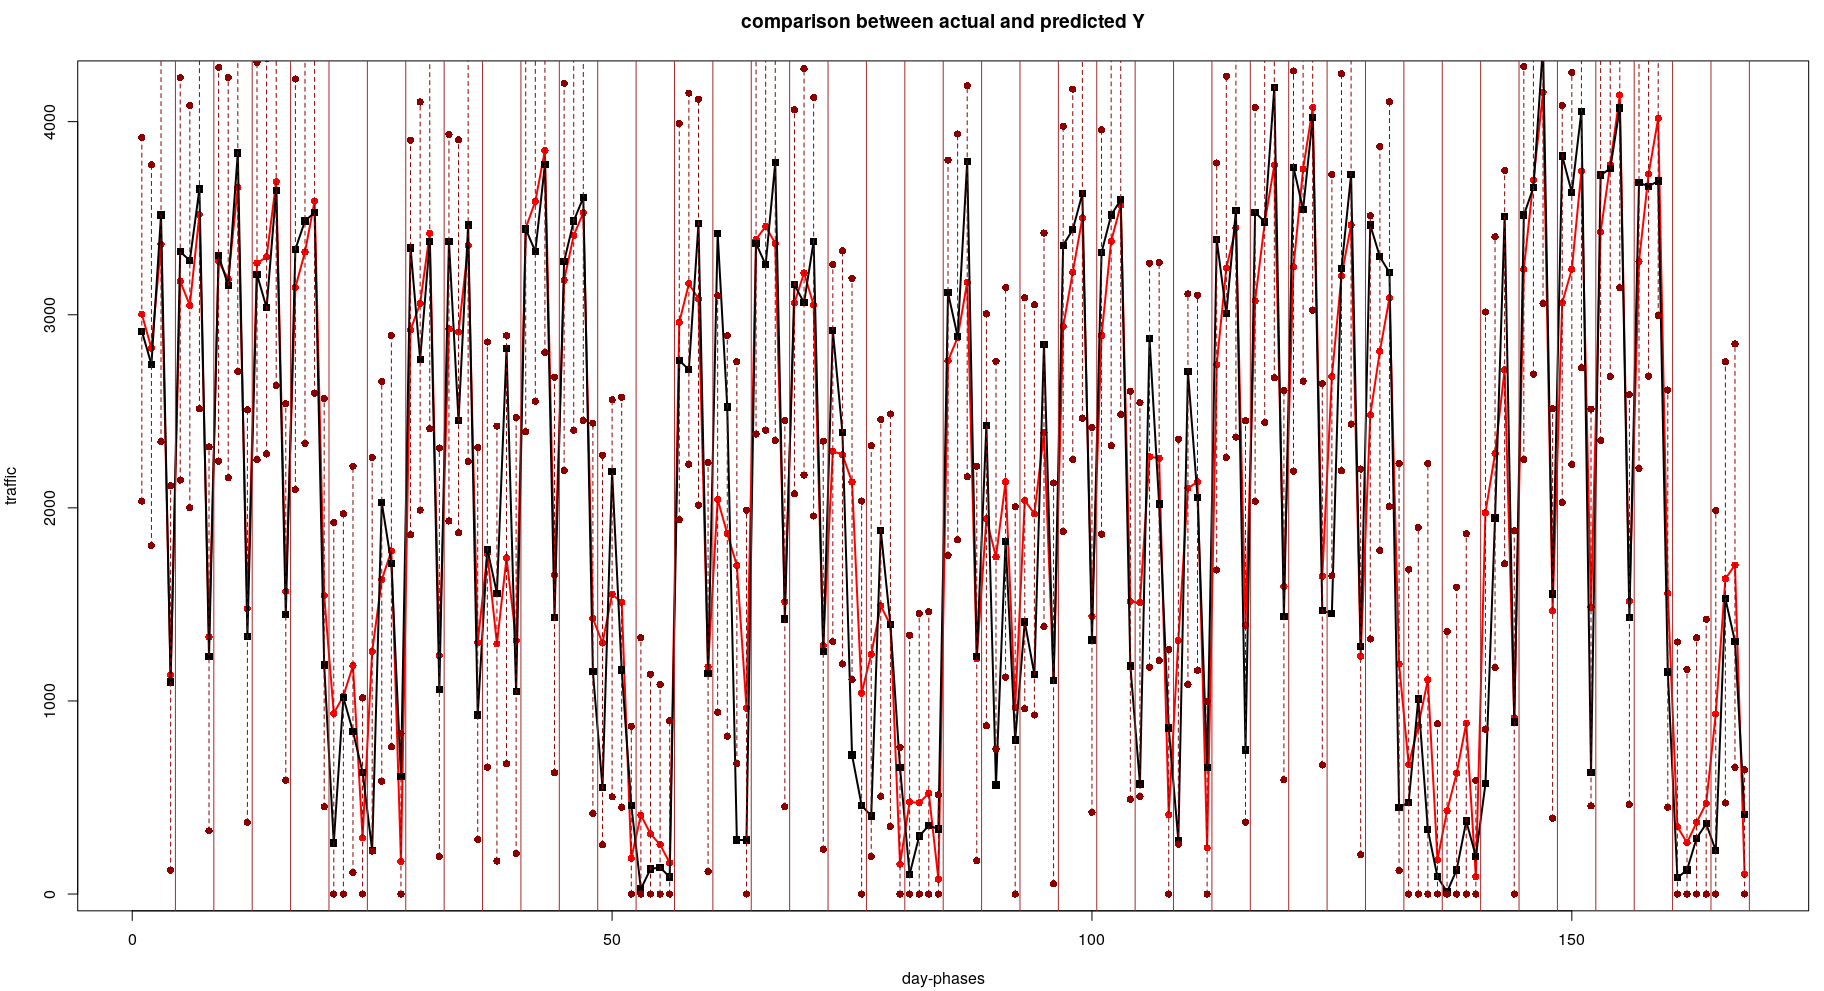
\includegraphics[width=140 mm]{pictures/Time_series.png}
	\caption{Global time series per slot}
	\label{fig:time series}
\end{figure}%



\chapter{Network model}
In this chapter we propose possible models to describe the "flux" of bicycle in clusters of stations. First dividing the stations in clusters as pre-processing with a modified version of the DBSCAN algorithm, then for every cluster the aim is to model the number of bicycles arriving and departing at stations belonging to the cluster: respectively $N^{IN}$ and $N^{OUT}$ in a certin time interval; we keep the division in days and time phases used in the BSTS. In this way the data are positive counts and the proposed models are \emph{Bivariate Poisson Two-Way Mixed GLMMs}.\\

\vspace{2mm}

For the rest of this chapter the $i$ index will distinguish the cluster, $t$ will be used for weekend and weekdays, and $h$ for the time phases of the day. And thus $i \in 1,...,N\_nodes$, $t = 1,2$ and $h = 1,...,H$. We will use the index $u$ to distinguish between the different data points: for example if the third row of the dataset ($u=3$) belongs to a weekend it will be indicated as $t(u)=2$; in this way two data points will have the same distribution (covariates notwithstanding) if $h(u_1) = h(u_2)$ and $t(u_1)=t(u_2)$. In all computations $H=4$ and the time phases are the same used for the BSTS model. The only two covariates that we will use are a dummy for the rain and the mean temperature for the day.
\section{Preprocessing}
On the columns there are the nodes (clusterized stations) and on the rows the evolving time with row index $u$. Clearly $h(u) = u \ \mathrm{mod}\ H$ and the belonging to weekends can be also extracted from $u$. We also wondered on the possible correlation between $N^{IN}$ and $N^{OUT}$ of the same node and time phase. 

\section{The Likelihood}
If we fix the indexes the random variables $(N^{IN}_{ith}, N^{OUT}_{ith})$ are	correlated. Therefore we decide to model them with a \emph{Bivariate Poisson}.
\subsection{Bivariate Poisson}
We say $(Y_1,Y_2) \sim \mathrm{BPo}(\lambda_0, \lambda_1, \lambda_2)$ if:
\begin{equation}
\begin{cases}
Y_j = X_0 + X_j \quad j = 1,2\\
X_j \sim \mathrm{Po}(\lambda_j) \quad j = 0,1,2
\end{cases}
\end{equation}
With the convention that $\mathrm{Po}(0) = \delta_0$, note that $\mathrm{Cov}(Y_1, Y_2) = \mathrm{Var}(X_0) = \lambda_0$.\\
 So $(N^{IN}_{it(u)h(u)}, N^{IN}_{it(u)h(u)}) \sim \mathrm{BPo}(\lambda^{(0)}_{it(u)h(u)}, \lambda^{(1)}_{it(u)h(u)}, \lambda^{(2)}_{it(u)h(u)})$ and the parameters of the model then are $(\lambda^{(0)}_{ith}, \lambda^{(1)}_{ith}, \lambda^{(2)}_{ith})$ and we will use for each of the three parameters the same hierarchical model.
\subsection{Zero Inflated Poisson}
We decided for a simple Poisson and not for a Zero Inflated Poisson for a purely computational reason, unfortunately the approximation revealed to bee too imprecise: the model fail to predict many zeros.

\begin{equation}
\begin{cases}
Y_j = \Gamma_j\delta_0 + (1-\Gamma_j)(X_0 + X_j) \quad j = 1,2\\
X_j \sim \mathrm{Po}(\lambda_j) \quad j = 0,1,2 
\end{cases}
\end{equation}

And implement a probit or logit link function for the $\Gamma_j$ parameters.

\section{Generalized Linear Two-Way Mixed Model}
As link function we choose the logarithm as is usual for a Poisson model. We deal with the division in weekdays/weekend and in the time phases in a similar way as a \emph{two-way ANOVA}, that is we consider the effect independent and sum the contributions. 

$$\gamma_{th}\cdot\mathbf{x} \rightarrow (\alpha_{t} + \beta_{h})\cdot\mathbf{x}$$

Conceptually this means that the effects influence the $\lambda$ parameter independently and there is a superposition of the effects of weekend and of the time phase.

Last we differentiate between two ways to deal with the nodal effect. 

\subsection{Offset model}
Taking inspiration from rate models with offsets we model the node effect as a multiplicative element that describes the size both in number of station per cluster and average number of travels. %Add more here as a description

\begin{equation}
\begin{cases}
\log(\lambda^{(j)}_{ith}) = (\boldmath{\theta^{(j)} +  \alpha^{(j)}_{t} + \beta_{h}^{(j)})}\cdot\mathbf{x} + \log(O_i)\\
\theta^{(j)}|a,B \stackrel{iid}{\sim} \mathcal{N}(a,B)\\
\alpha_{t}^{(j)}|\Sigma^{(j)} \stackrel{iid}{\sim} \mathcal{N}(0, \Sigma)\\
\beta_{h}^{(j)}|\Omega^{(j)} \stackrel{iid}{\sim} \mathcal{N}(0, \Omega)\\
a \sim \mathcal{N}(a_0, A_0)\\
B \sim invWishart(B_0, p+1)\\
\Sigma, \Omega \stackrel{iid}{\sim} invWishart(C_0, p+1)

\end{cases}
\end{equation}

%Riprendi come da slides di bayesiana il ruolo del mixed

There is the problem of deciding the offsets $O_i \in \mathbb{R}^+$, which give a measure of the "size" of the cluster both in number of stations and in bicycle traffic. For our computation we decided on a somehow suboptimal choice: 
$$O_i = \mathrm{Avg}(N^{IN}_i + N^{OUT}_i)$$

The offset is the average of traffic in the cluster, this creates a sort of circular dependency where we use the data to fit the data. We mitigated this by taking the average only on the first third of the dataset. In a real application one could divide the period in two, one to compute the offsets and the other to fit the model. We decided against this because the number of data points provided is already small.

\subsection{Model with parametric offsets (PO model)}
While we considered the offsets known in the previous model, we now group them with the other parameters.

\begin{equation}
\begin{cases}
\log(\lambda^{(j)}_{ith}) = (\boldmath{\theta^{(j)} +  \alpha^{(j)}_{t} + \beta_{h}^{(j)})}\cdot\mathbf{x} + \Phi_i\\
\theta^{(j)}|a,B \stackrel{iid}{\sim} \mathcal{N}(a,B)\\
\alpha_{t}^{(j)}|\Sigma^{(j)} \stackrel{iid}{\sim} \mathcal{N}(0, \Sigma)\\
\beta_{h}^{(j)}|\Omega^{(j)} \stackrel{iid}{\sim} \mathcal{N}(0, \Omega)\\
\Phi_i \stackrel{iid}{\sim} \mathcal{N}(\Phi_0, F_0)\\
a \sim \mathcal{N}(a_0, A_0)\\
B \sim invWishart(B_0, p+1)\\
\Sigma, \Omega \stackrel{iid}{\sim} invWishart(C_0, p+1)

\end{cases}
\end{equation}

Where the $\Phi_i \in \mathbb{R}$ take the role of $\log(O_i)$. The implicit belief of the model is that the $\Phi_i$, taking the role of a "size" parameter, does not depend on $j$; that is it has the same effect on both the inward and outward flux and their correlation. In this way it has the exact same role of the offsets and we will be able to compare the two.

\section{Computation of the posterior with JAGS software}
We used the package rjags to sample from the posterior of the $(\alpha_{t}^{(j)}, \beta_{h}^{(j)}, \theta^{(j)}, \Phi_i)$ parameters. Both models are computationally heavy, for this reason we had to limit the number of chains to 3 with 10000 iterations for the adaptation, 19000 for the burn-in and only 1000 effective sampling iterations, taken one every 10. It's important to notice that not unlike a two-way ANOVA the models are not identifiable with respect to all parameters. Indeed only the sum $(\boldmath{\theta^{(j)} +  \alpha^{(j)}_{t} + \beta_{h}^{(j)})}$ with $t,h$ fixed has a meaning in itself. Even taking this into account, the results are unsatisfactory: in particularly regarding the adaptation, with the three chains stabilizing on three different values. Moreover the autocorrelation is too high in the offsets model, while being more acceptable in the PO model. \\

\begin{figure}[H]
	\begin{subfigure}[H]{.5\linewidth}
		\centering
		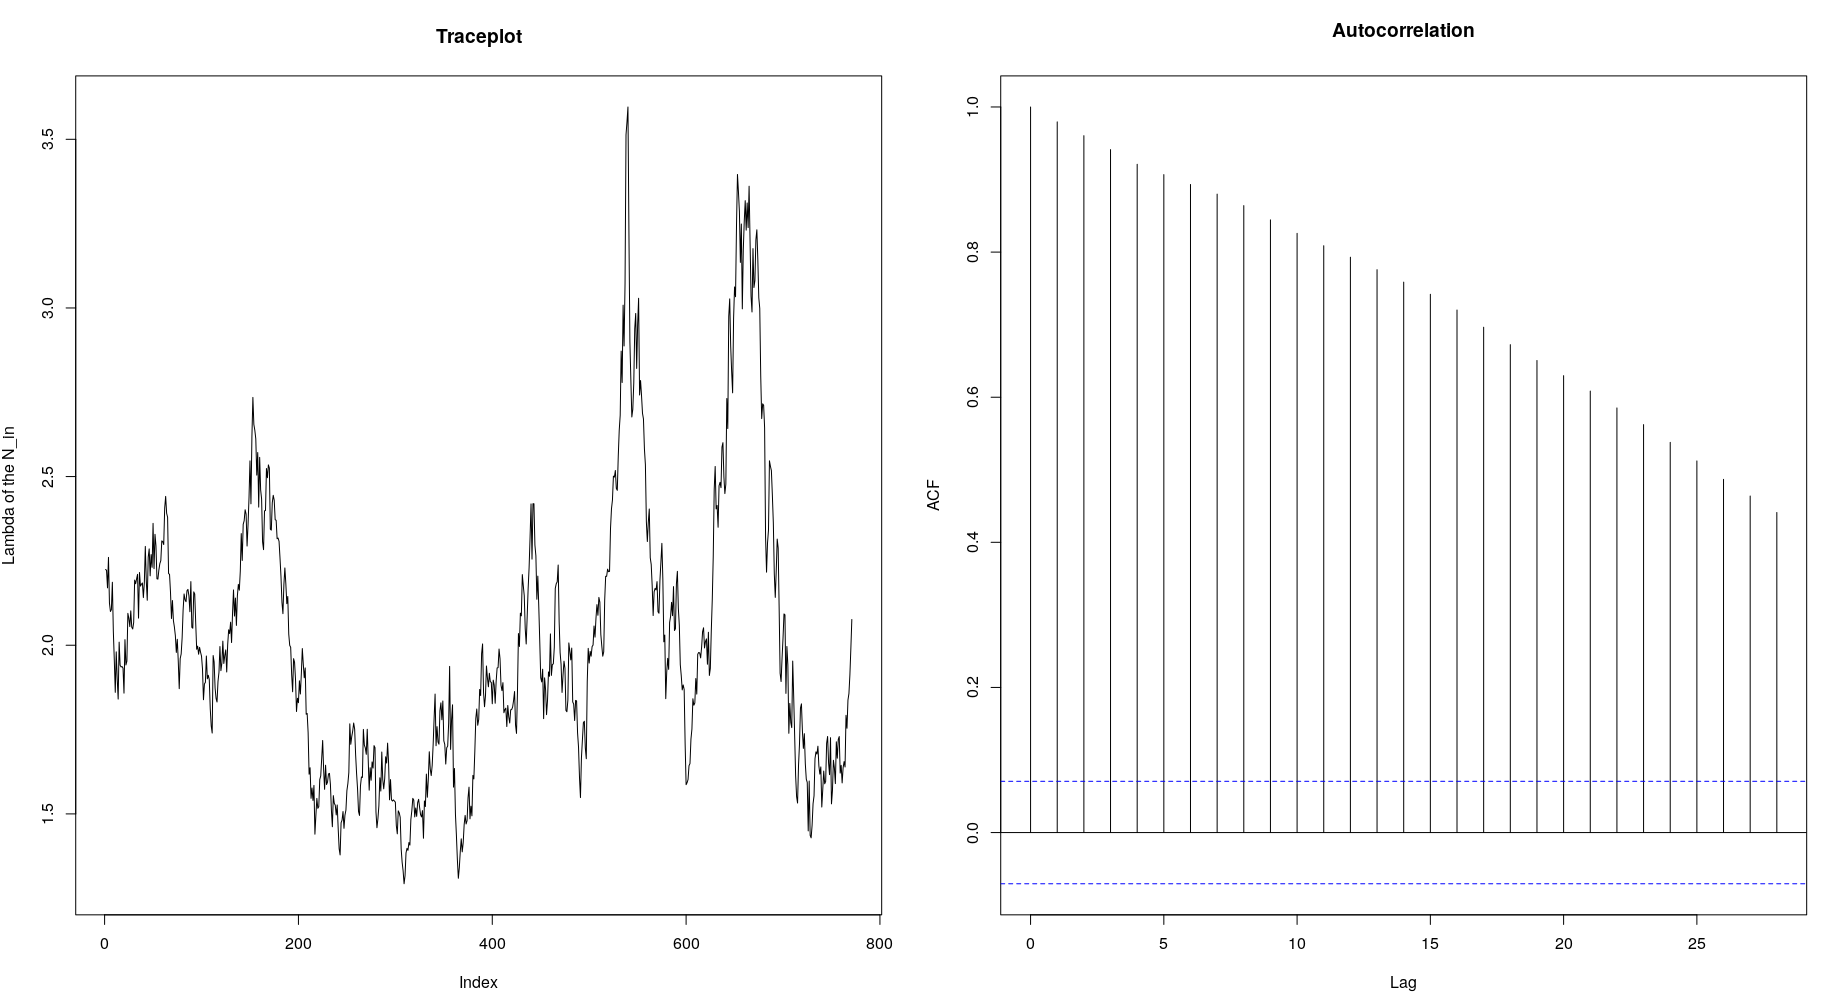
\includegraphics[width=70 mm]{pictures/posterior_off.png}
		\caption{For the offsets model}
		\label{fig:post_off}
	\end{subfigure}
	\hfill
	\begin{subfigure}[H]{.5\linewidth}
		\centering
		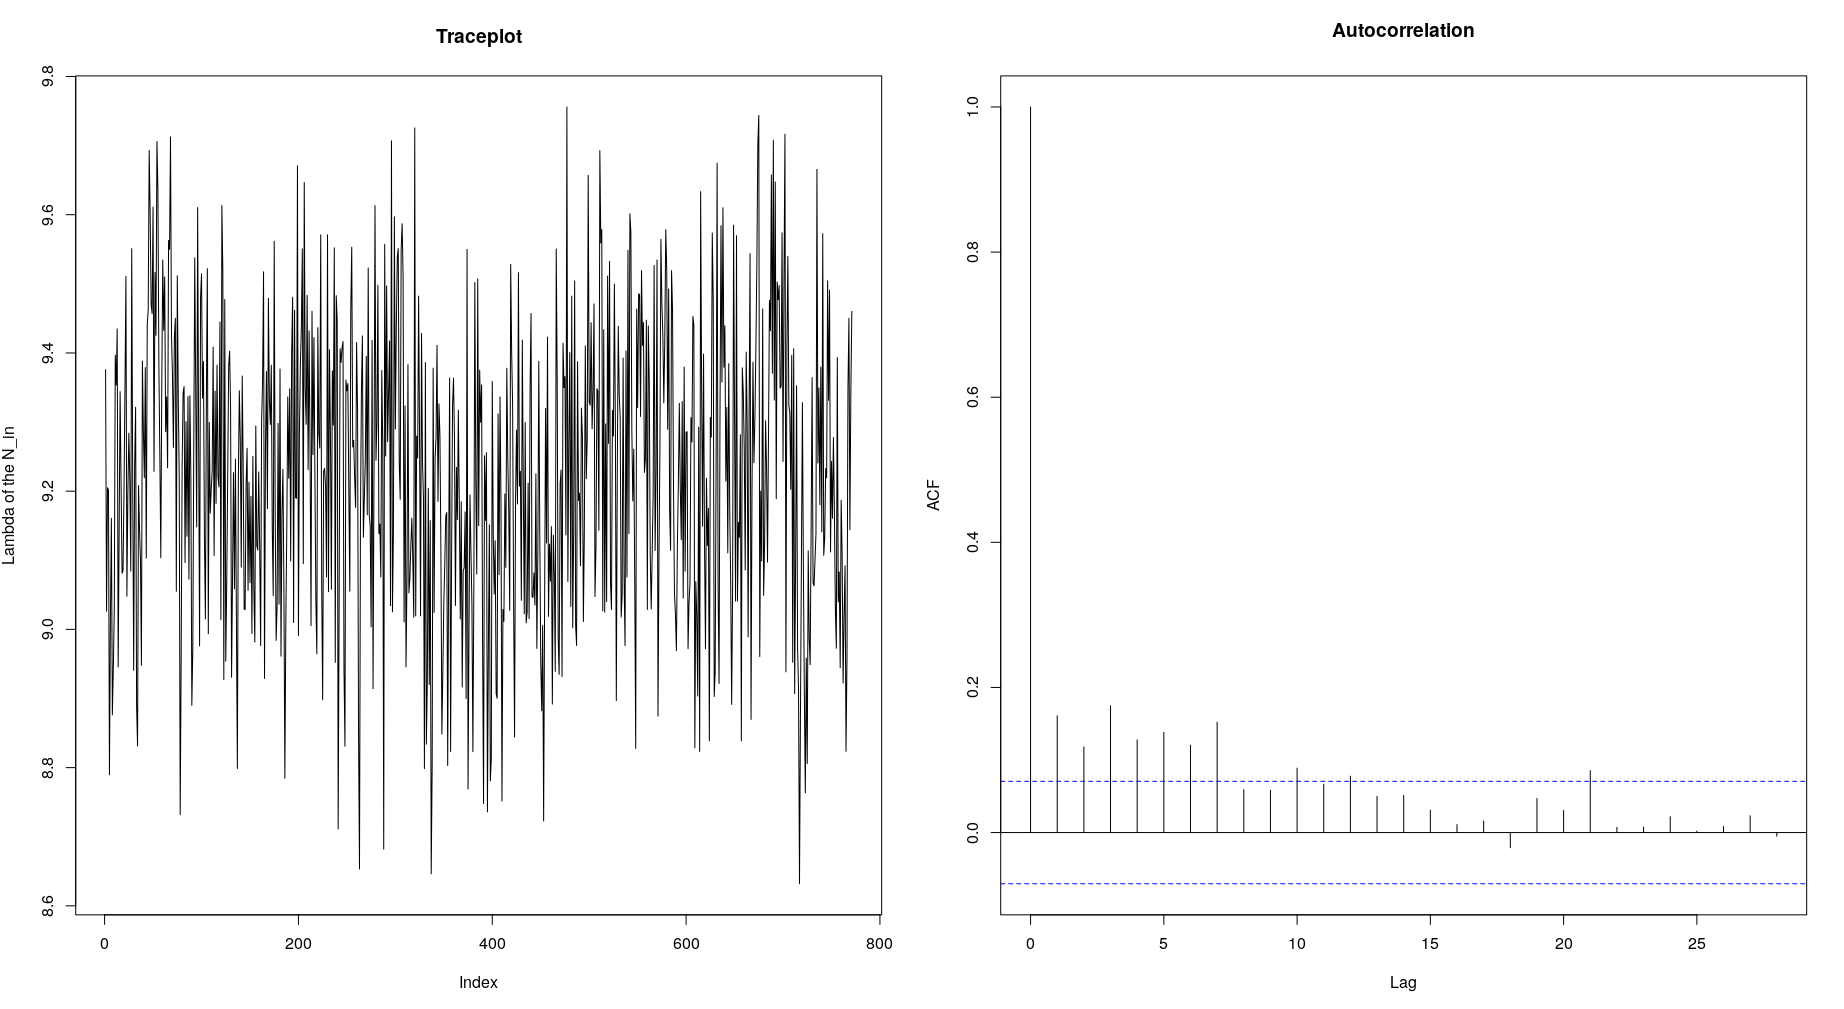
\includegraphics[width=70 mm]{pictures/posterior_nbn.png}
		\caption{For the PO model}
		\label{fig:post_nbn}
	\end{subfigure}%
	\caption{Results produced by the model}
\end{figure}


The predictiveness of both models is quite bad, with more than half of the data outside of their 95\% predictive intervals.

\begin{center}
	\begin{tabular}{ |c|c|c| } 
		\hline
		& $N^{IN}$ & $N^{OUT}$ \\ 
		\hline
		Offsets & 41.0\% & 62.2\% \\ 
		PO & 39.7\% & 38.6\% \\ 
		\hline
	\end{tabular}
\end{center}

Example of a simple table


We believe it might be because the JAGS chain could not reach stationarity, unfortunately we could run the chain for longer due to the computations being too time consuming. \\

\begin{figure}[H]
	\centering
	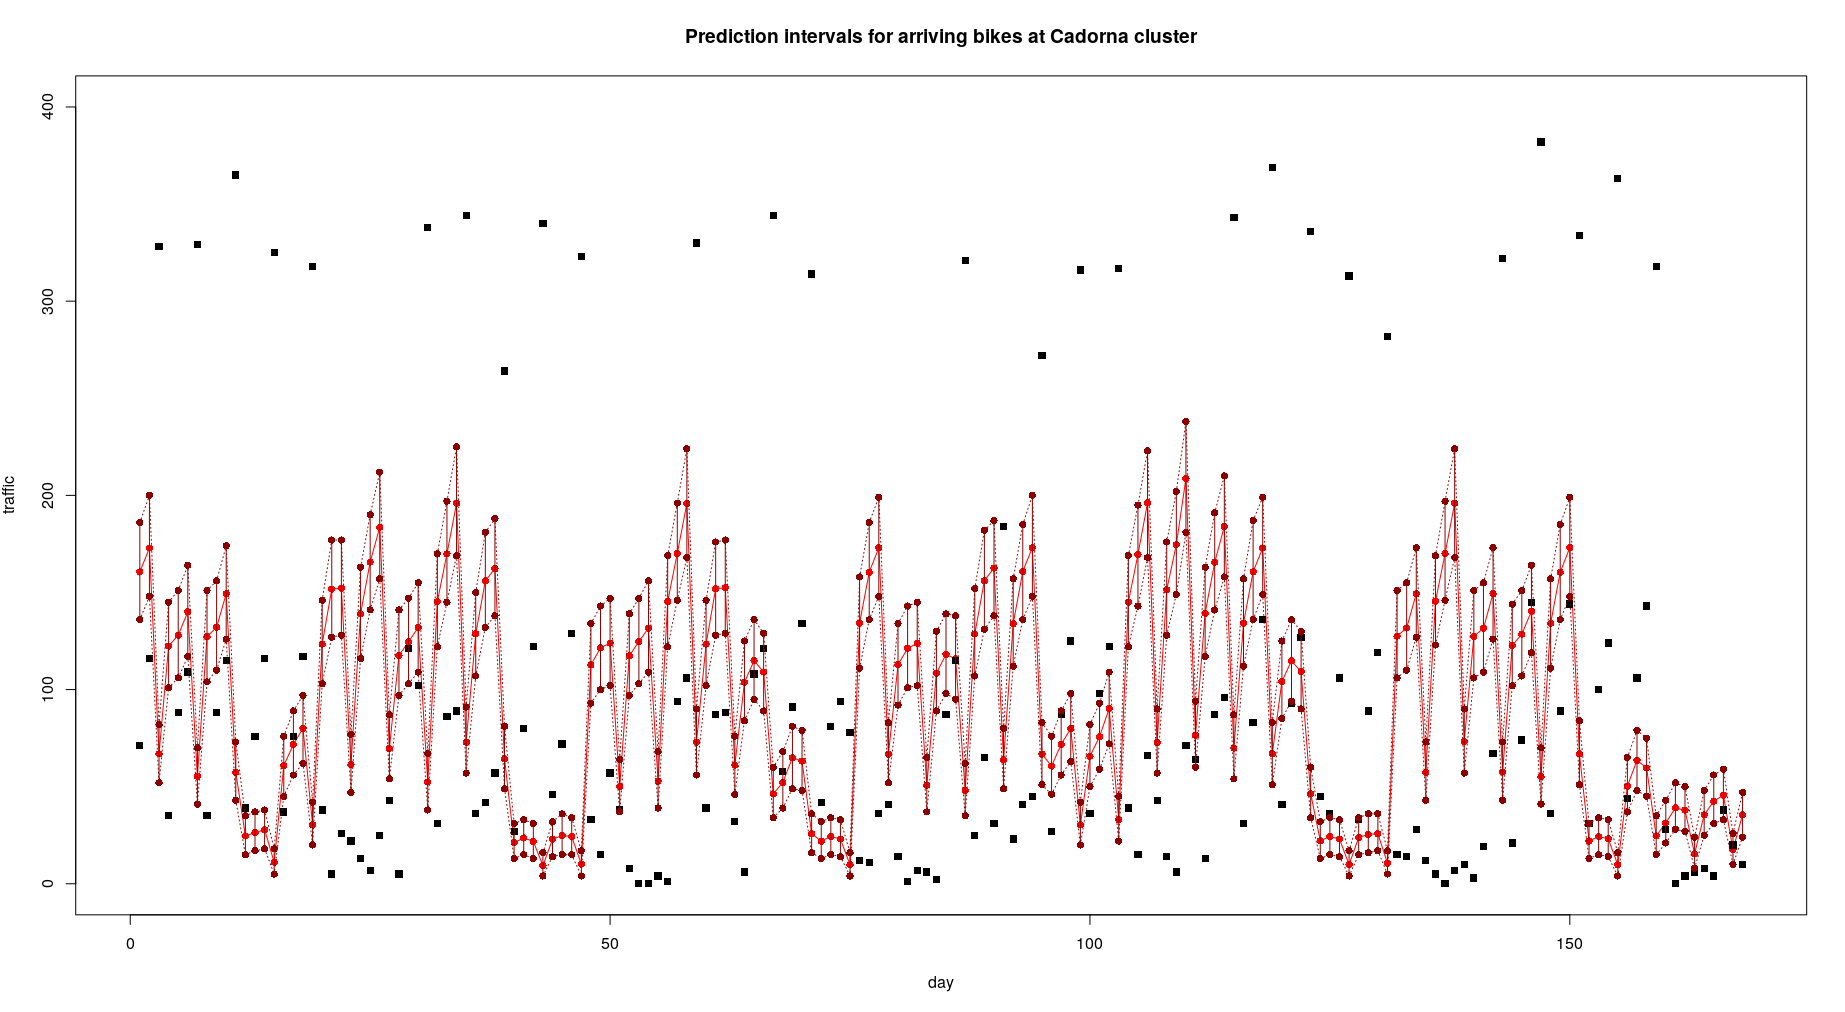
\includegraphics[width=120 mm]{pictures/cadorna_nin.png}
	\caption{}
	\label{fig:network_pred}
\end{figure}

There are also other possibilities: inspecting the plot \ref{fig:network_pred} of the prediction intervals we notice that there are two main categories of data points that the model systematically forecasts erroneously. The first are the zeros, which are more common in small nodes. The second case are "counter-nodes", clusters that behave in contrast with the others. For examples clusters near a big train station will see a net outward flux during the morning when commute workers leave the station, while other stations see a net inward flux of the same people arriving. Considering this, a possible generalization would be to employ a Zero Inflated Poisson likelihood and adding a two groups mixture effect of the time phase in the node $\beta_{t,i}$. 

\section{A final spatial model}
Instead of modeling a bivariate Poisson through a fictitious common covariance term, with this approach we put the dependence at lower level still trying to  exploit the graph structure. We divide the nodes into $M$ groups. Notation: $ g(i) $ will denote the cluster of node $ i $ (classified through a mixture $ \delta(i) $ attribution variable), $ w(t) $ means if day $ t $ is weekend or weekday (mixed effect component).

\begin{model} Mixed loglinear-BSTS\\
\begin{equation*}
\begin{aligned}
&\textsc{Model}\\
&(N^{IN}, N^{OUT})_{ith}\sim Zip(\pi_{g(i)},\lambda_{ith}^{IN})\otimes Zip(\pi_{g(i)},\lambda_{ith}^{OUT})\\
&\log(\lambda^{j}_{ith}) = \mu^{j}_{ith}+\boldsymbol{\beta}^j_{g_iw_th}\mathbf{z}_t + \epsilon_{ith}^j\\
&\mu_{ith}^{IN} = \frac{1}{2} \mu^{IN}_{i(t-S)h} + \frac{1}{2} \frac{\sum_{j \in \mathcal{N}} \phi^{IN}_{ij}\mu_{jt(h-1)}^{OUT}}{\sum_{j \in \mathcal{N}} \phi^{IN}_{ij}}\\
&\mu_{ith}^{OUT} = \frac{1}{2} \mu^{OUT}_{i(t-S)h} + \frac{1}{2} \frac{\sum_{j \in \mathcal{N}} \phi^{OUT}_{ij}\mu_{jth}^{IN}}{\sum_{j \in \mathcal{N}} \phi^{OUT}_{ij}}\\
\end{aligned}
\qquad \qquad
\begin{aligned}[c]
&\textsc{Priors}\\
&\pi_{g(i)} \sim Be(p_{g(i)})\\
&\boldsymbol{\beta} \sim \mathcal{N}(\mathbf{0},\boldsymbol{\Sigma})\\
&\mathbf{\delta}_i \sim \mathrm{Dir}(a_1,...,a_M)
\end{aligned}
\end{equation*}
\end{model}

$ \phi_{ij}^* $ is a deterministic coefficient that takes into account both the distace of node $ j $ from $ i $ and the magnitude (IN or OUT) of the node $ j $, for instance we might select $ \phi_{ij}^*=\frac{s^*_j}{d_{ij}} $ where $ d_{ij} $ is the distance between node $ i $ and $ j $ and $ s_j^* $ is the (inner or outer) strength of $ j $. $ p_{g(i)} $ are also hyperparameters and their value is in (0,1), we can suppose a non-informative prior for vector $ \mathbf{p} $, or put all the coefficients to the same value. Finally, $ \boldsymbol{\delta} $ is the attribution parameter, that links each node to its cluster. We can suppose a Dirichlet prior for it, endowed with some uninformative parameter $ \mathbf{a} $. 

\appendix
\chapter{Bibliography}
\begin{itemize}[noitemsep,topsep=0pt,parsep=0pt,partopsep=0pt,labelwidth=1.4cm,align=left,itemindent=0cm]
	\item[{[BG19]}] G. Bissoli, C. Principi, G. M. Rinaldi, M. Beraha and
	A. Guglielmi (2019),\\ $ \textit{A Bayesian model for network flow data: an application to BikeMi trips} $\\ SIS 2019 - Smart Statistics for Smart Applications, conference proceeding pages	673 - 678.
	\item[{[TPV19]}] A. Torti, A. Pini, S. Vantini (2019),\\ $ \textit{Modeling time-varying mobility flows using function-on-
	function regression:}\\ \textit{analysis of a bike sharing system in the city of Milan} $\\ Tech. rep., MOX, Politecnico di Milano.
	\item[{[BD02]}] P. J. Brockwell, R. A. Davis (2002),\\ $ \textit{Introduction to Time Series and Forecasting, Second Edition} $\\ Springer Texts in Statistics, pages 31 - 35.
	\item[{[SV13]}] S. L. Scott,
	H. Variani (2013),\\ $ \textit{Predicting the Present with Bayesian Structural Time Series} $.
	\item[{[JRN18]}] J. Qiu, S. Rao Jammalamadaka, 
	N. Ning (2018),\\ $ \textit{Multivariate Bayesian Structural Time Series Model} $,\\Department of Statistics and Applied Probability,
	University of California.
	\item[{[VGG16]}] A. Vehtari, A. Gelman, J. Gabry (2016),\\ $ \textit{Practical Bayesian model evaluation using leave-one-out cross-validation and WAIC} $.
\end{itemize}

\end{document}
